\documentclass{beamer}
\mode<presentation>
\usepackage{amssymb,textcomp}
%\usepackage{beamerthemesplit}
\usepackage{beamerthemeJuanLesPins}
\usepackage{verbatim}
\usepackage{algorithm2e}
\usepackage{subfigure}
\usefonttheme{serif}
\title{Unidad II: Soluci\'on Num\'erica de Ecuaciones No Lineales.}
\author{Jos\'e Luis Ram\'irez B.}
\date{\today}

\begin{document}

\frame{\titlepage}

\frame{\tableofcontents}

\section{Introducci\'on}
\begin{frame}[fragile]
  \frametitle{Motivaci\'on.} 
  \begin{itemize}
    \item<1-> La determinaci\'on de las ra\'ices de una ecuaci\'on o de un sistema de ecuaciones, es uno de los problemas m\'as antiguos de aproximaci\'on num\'erica que se presenta con frecuencia en la soluci\'on de una gran variedad de problemas en la matem\'atica aplicada.
    \item En un problema m\'as general, si $f$ es una funci\'on cualquiera, la ecuaci\'on $f(x)=0$ no puede resolverse anal\'iticamente. De hecho, ni siquiera se sabe a priori cu\'antos ceros tiene $f$: ?`varios, uno, ninguno? 
  \end{itemize}    
\end{frame}
%%%%%
\frame
{
  \frametitle{Motivaci\'on.}
 La ecuaci\'on de Peng-Robinson es una ecuaci\'on de
estado que proporciona la presi\'on $P$ de un gas mediante:
  \begin{equation}
   P=\frac{R*T}{V-b}- \frac{a}{V*(V+b)+b*(V-b)}
  \end{equation}

donde $a$ y $b$ son constantes, $T$ es la temperatura absoluta a la que se encuentra el gas, $V$ es el volumen espec\'ifico y $R$ es la constante de los gases perfectos ($8.31441 J/(mol.^\circ K)$). Para el $CO_2$ las constantes $a$ y $b$ toman los valores $a=364.61 m^6.kPa/(kg.mol)^2$ y $b=0.02664 m^3/kg.mol$. Supongamos que se desea encontrar la densidad ($1/V$) del $CO_2$ a una presi\'on de $10^4 kPa$ y a una temperatura de $340^\circ K$ usando la ecuaci\'on de Peng- Robinson.
}
%%%
%%%%
\frame{
Dos casos importantes:
\begin{enumerate}
 \item<2-> Soluci\'on de una ecuaci\'on no lineal con una inc\'ognita, donde:
 $$
 f:\mathbb{R}\to\mathbb{R}
 $$
 La soluci\'on es un escalar $x$ para el cual $f(x)=0$
 \item<3-> Soluci\'on a un sistema acoplado de $n$ ecuaciones no lineales en las $n$ inc\'ognitas, donde:
 $$
 f:\mathbb{R}^{n}\to\mathbb{R}^{n}
 $$
 La soluci\'on es un vector $x$ para el cual todas las componentes de $f$ son cero simult\'aneamente, $f(x)=0$
\end{enumerate}
}
%%%%
\frame{
Ejemplos:
\begin{enumerate}
 \item<2-> Ecuaci\'on no lineal en una dimensi\'on
 $$
 x^{2}-4\sin(x)=0
 $$
 para la cual $x=1.9$ es una soluci\'on aproximada.
 \item<3-> Sistema de ecuaciones no lineales en dos dimensiones
 $$
 \left\{\begin{array}{rcl}
         x_1^{2}-x_2+0.25 & = & 0\\
         -x_1+x_2^{2}+0.25 & = & 0
        \end{array}
\right.
 $$
 para el cual el vector soluci\'on es $x=[0.5, 0.5]^{t}$
\end{enumerate}

}
%%%%
\frame{
\frametitle{Ejemplo: Una dimensi\'on}
Ecuaciones no lineales pueden tener cualquier n\'umero de soluciones
\begin{itemize}
 \item<2-> $e^{x}+1=0$ no posee soluci\'on.
 \item<3-> $e^{-x}-x=0$ tiene una soluci\'on.
 \item<4-> $x^{2}-4\sin(x)=0$ posee dos soluciones.
 \item<5-> $x^{3}+6x^{2}+11x-6=0$ posee tres soluciones.
 \item<6-> $\sin(x)=0$ posee infinitas soluciones.
\end{itemize}
}
%%%%
\frame
{
\frametitle{El M\'etodo Gr\'afico}
El m\'etodo gr\'afico es un m\'etodo muy simple, consiste en calcular valores de la variable dependiente para distintos
valores de la variable independiente, para luego observar el punto de intersecci\'on de la funci\'on con el eje de las
abscisas. Este punto proporciona una primera aproximaci\'on a la ra\'iz de la ecuaci\'on.
\begin{center}
  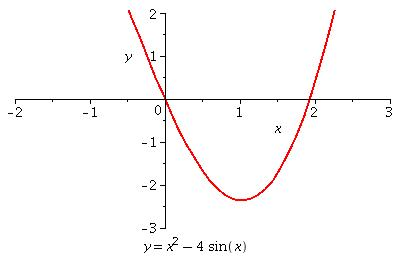
\includegraphics[scale=0.5]{eq2sol.jpg}
 \end{center}
}
%%%
\frame
{
\frametitle{Soluci\'on de Ecuaciones No Lineales}

\begin{block}{Definici\'on}
Sea $f:\mathbb{R} \rightarrow \mathbb{R}$ una funci\'on no lineal. Se llama ra\'iz o cero de la ecuaci\'on no lineal $f(x)=0$ a todo valor $\alpha \in \mathbb{R}$ tal que $f(\alpha)=0$.

\end{block}

Se podr\'ian precisar tres etapas en el c\'alculo de un cero:

\begin{itemize}
\item<1-> Localizaci\'on: Existencia de las ra\'ices.
\item<2-> Separaci\'on: Aislar ra\'ices en caso de la existencia de varias.
\item<3-> Aproximaci\'on Num\'erica: Generaci\'on de una sucesi\'on convergente a la ra\'iz $\alpha$.
\end{itemize}
}
%%%%
\frame
{
\frametitle{Soluci\'on de Ecuaciones No Lineales}
\begin{block}{Definici\'on}
  Sea $f : \mathbb{R} \to \mathbb{R}$ una funci\'on, $\alpha \in \mathbb{R}$ es un cero de $f$ de multiplicidad $p \in \mathbb{Z}$, si
$$
f(x)=(x-\alpha)^pq(x)
$$
con $q(\alpha)\neq 0$.
\end{block}

\uncover<2->{
Si $f(\alpha)=f'(\alpha)=f''(\alpha)=\cdots=f^{(m-1)}(\alpha)=0$ pero $f^{(m)}(\alpha)\neq0$, entonces la ra\'iz $\alpha$ posee multiplicidad $m$}
}
%%%%
\section{Ratas de Convergencia}
\frame
{
 \frametitle{Ratas de Convergencia}
Suponiendo que un m\'etodo iterativo produce una sucesi\'on de puntos $x_1, x_2,x_3,\ldots$ a partir de un punto inicial $x_0$. Se
quiere conocer si converge a la soluci\'on $\alpha$ y cual es la rapidez con que lo hace.
\begin{block}{Definici\'on}
  La sucesi\'on $\{x_n\} \subset \mathbb{R}$ converge a $\alpha \in \mathbb{R}$ si
$$
\lim_{n\to\infty}|x_n -\alpha|=0
$$
Sea $e_n = x_n - \alpha$. Si existen dos constantes $\lambda > 0$ y $r > 0$ tales que
$$
\lim_{n \to \infty}\frac{|e_{n+1}|}{|e_n|^{r}}=\lambda
$$
se dice que $\{x_n\}$ converge hacia $\alpha$, con orden de convergencia $r$ y $\lambda$ se denomina la constante asint\'otica del
error..
\end{block}
}
%%%%
\frame{
 \frametitle{Ratas de Convergencia}
Algunos casos de inter\'es
\begin{itemize}
 \item<2-> $r=1$: lineal ($\lambda<1$)
 \item<3-> $r>1$: superlineal
 \item<4-> $r=2$: cuadr\'atico
\end{itemize}
\uncover<5->{
\begin{center}
 \begin{tabular}{p{2.7cm}|p{3cm}}
  Rata de Convergencia & D\'igitos ganados por iteraci\'on\\ \hline
  lineal & constante\\
  superlineal & increment\'andose\\
  cuadr\'atica & doble
 \end{tabular}
\end{center}}
}
%%%%
\section{M\'etodo de Bisecci\'on}
\frame{
 \frametitle{M\'etodo de Bisecci\'on}
 \begin{block}{Teorema del valor intermedio de Bolzano.}
  Supongamos que $f \in C [a, b]$ y que $L$ es cualquier n\'umero
  entre $f(a)$ y $f(b)$. Entonces existe un n\'umero $c$ en $(a,b)$ tal que $f(c) = L$.
  \end{block}
}
%%%%%
\frame{
  \frametitle{M\'etodo de Bisecci\'on}
  \begin{itemize}
    \item <1-> Supongamos que $f$ es una funci\'on continua en un intervalo $[a,b]$, y $f(a)\cdot f(b) < 0$. Entonces, por el Teorema de Bolzano, existe al menos un $p \in (a,b)$, tal que $f(p) =0$.
    \item <2-> Una primera aproximaci\'on de este punto $p*$ puede ser el punto medio:
    \begin{block}{}
           $$p_1=\frac{a+b}{2}$$
    \end{block}
  \end{itemize}
}
%%%%
\frame{
  \frametitle{M\'etodo de Bisecci\'on}
  \begin{itemize}
  \item<1->Dado que la funci\'on es continua, si $f(a) \cdot f(p_1) < 0$ en el intervalo $[a,p_1]$ habr\'a al menos una soluci\'on de la ecuaci\'on.
  \item<2-> Y si $f(a)\cdot f(p_1) > 0$ en el intervalo $[p_1,b]$ existir\'a al menos una ra\'iz.
  \item<3->Por tanto se habr\'a definido un nuevo intervalo $[a_1,b_1]$ en el que existir\'a una soluci\'on. Al que puede aplic\'arsele nuevamente el proceso anterior.
  \end{itemize}
}
%%%%
\frame{
 \frametitle{M\'etodo de Bisecci\'on}
En general, partiendo de un intervalo $[a_j,b_j]$ en el que $f(a_j)\cdot f (b_j) < 0$ se denotar\'a por $p_{j+1}$ al punto medio del intervalo:

\begin{block}{}
$$p_{j+1} =\frac{a_j + b_j}{2}$$
\end{block}
procediendo de la forma siguiente:
\begin{itemize}
  \item<1-> Si $f(p_{j+1}) = 0$ se habr\'a obtenido una soluci\'on de la ecuaci\'on: el punto $p_{j+1}$.
  \item<2-> Si $f(a_j)\cdot f(p_{j+1})<0$ se denotar\'a por: $a_{j+1} = a_j$ y por $b_{j+1} = p_{j+1}$.
  \item<3-> Si $f(a_j)\cdot f(p_{j+1})>0$ se denotar\'a por: $a_{j+1} = p_{j+1}$ y por $b_{j+1} = b_j$.
  \item<4-> Al nuevo intervalo $[a_{j+1},b_{j+1}]$ se le vuelve a aplicar el mismo proceso.
\end{itemize}
}
%%%%
 \frame{
 \centering
 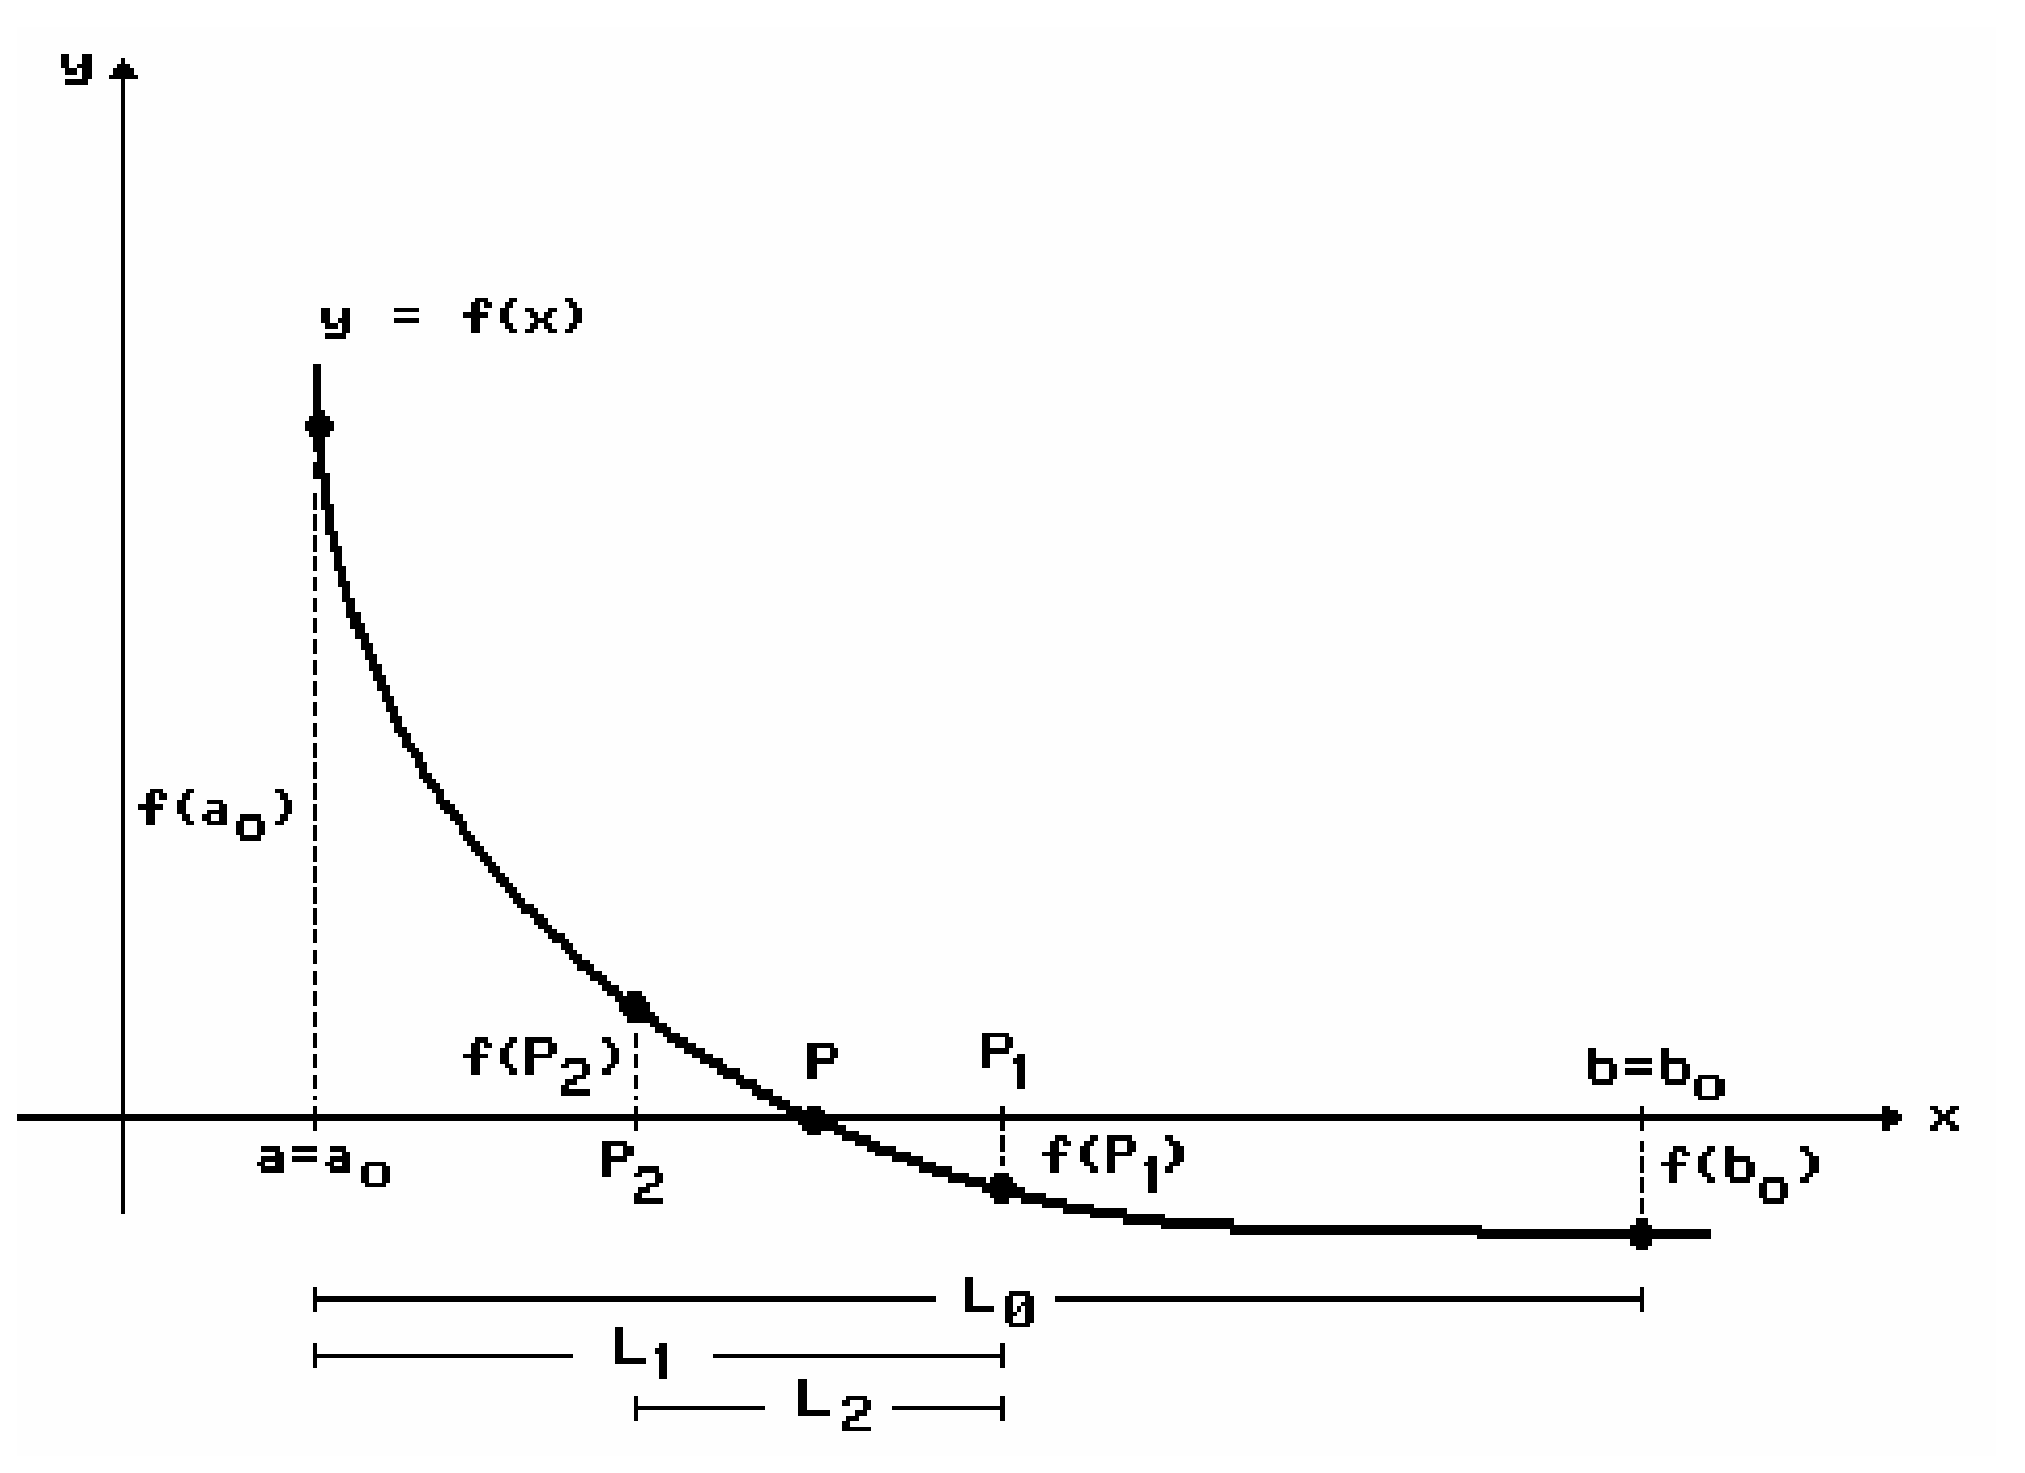
\includegraphics[scale=0.35]{bisec.eps}
 }
%%%%%
\begin{frame}
  \frametitle{M\'etodo de Bisecci\'on}
  \begin{block}{Teorema}
    Sea $f$ continua en $[a, b]$, tal que $f (a)f (b) < 0$. Si $[a_1 , b_1 ], [a_2 , b_2 ], \ldots , [a_n , b_n ]$, denota
los intervalos obtenidos por el m\'etodo de bisecci\'on entonces existen
$$
\lim_{n \to \infty} a_n \qquad \lim_{n \to \infty}b_n
$$
son iguales y convergen a un cero de $f$ . M\'as a\'un, definiendo $c_n =\frac{b_n +a_n}{2}, \, \exists 
\displaystyle\lim_{n \to \infty} c_n = \alpha$, con $f (\alpha) = 0$ y se verifica
$$
|\alpha - c_n| \leq \frac{b-a}{2^n}, \quad \forall n \in \mathbb{N}
$$
  \end{block}
\end{frame}
%%%%
\frame{
  \frametitle{M\'etodo de Bisecci\'on}
  \begin{block}{Demostraci\'on}
    \begin{itemize}
      \item<1-> Por definici\'on se tiene que $a\leq a_1 \leq a_2 \leq \cdots a_n \leq \cdots \leq b$ luego $a_n$ es una sucesi\'on creciente y acotada superiormente por lo tanto es convergente. De manera an\'aloga resulta convergente la sucesi\'on $b_n$ por ser decreciente y acotada inferiormente.
      \item<2-> Sean $\displaystyle a^* = \lim_{n \to \infty} a_n$ y $\displaystyle b^* = \lim_{n \to \infty} b_n$ . Se quiere probar que $a^* = b^*$ o lo que es
      equivalente que $\displaystyle\lim_{n \to \infty} b_n - a_n = 0$. Se observa que
      $$
      b_n - a_n = \frac{b_{n-1}-a_{n-1}}{2} = \cdots = \frac{b_1 - a_1}{2^{n-1}}\, \xrightarrow{n \to \infty} \, 0
      $$
    \end{itemize}
  \end{block}
}
%%%%
\frame{
  \frametitle{M\'etodo de Bisecci\'on}
  \begin{block}{Demostraci\'on}
    \begin{itemize}
      \item Definiendo $\alpha = a^* = b^*$, falta probar que $f (\alpha) = 0$. Se sabe que $f (a_n )f (b_n ) \leq 0 \, \forall n
      \in \mathbb{N}$, luego como $f \in C([a, b])$ se tiene que
      $$
      \begin{array}{l}
        \underbrace{\lim_{n \to \infty}f(a_n)}_{f(\alpha)} \underbrace{\lim_{n \to \infty}f(b_n)}_{f(\alpha)} = \displaystyle\lim_{n \to
      \infty}f(a_n)f(b_n) \leq 0\\
      \Rightarrow f^2(\alpha) \leq 0 \Rightarrow f(\alpha) = 0
      \end{array}
      $$      
      Adem\'as 
      $$
      |\alpha - c_n|\leq \left|\frac{b_n-a_n}{2}\right| = \frac{b_n-a_n}{2} = \frac{b-a}{2^n}
      $$
      como se quer\'ia probar.
      
    \end{itemize}
  \end{block}
}
%%%%%
\frame{
  \frametitle{M\'etodo de Bisecci\'on}
  \begin{block}{Proposici\'on}
    \begin{itemize}
      \item<1-> Si la funci\'on $f(x)$ es continua y estr\'ictamente mon\'otona en el intervalo $[a, b]$ y adem\'as es tal que
$f(a)\cdot f(b) < 0$, dado un valor real positivo $\delta$ y denotando por $N$ al menor n\'umero natural tal que:
$$
N > \frac{\ln\left(\frac{|b-a|}{\delta}\right)}{\ln(2)}
$$
se verifica que $N$ iteraciones del proceso de bisecci\'on conducen a un valor $x_{N+1}$ que dista de la soluci\'on de la ecuaci\'on $f (x) = 0$ una magnitud inferior a $\delta$.
    \end{itemize}
  \end{block}
}
%%%%%
\begin{frame}
  \frametitle{M\'etodo de Bisecci\'on}
  \small{
  \begin{algorithm}[H]
    %\SetLine
    \SetKwInOut{Input}{input}
    \SetKwInOut{Output}{output}
    \caption{Algoritmo de Bisecci\'on.}
    \Input{$a,b \in \mathbb{R}$, M\'aximo de iteraciones $N$, tolerancia $TOL$.}
    \Output{Soluci\'on aproximada $p$ tal que $f(p) \approx 0$.}
    %\BlankLine
    $i \leftarrow 1$\\
    \While{$i \leq N$}
    {
     $\displaystyle p \leftarrow a + \frac{b-a}{2} = \frac{b+a}{2}$\\
     $i \leftarrow i +1$\\
     \If{$|f(p)|<TOL \vee \displaystyle\frac{b-a}{2}<TOL$}
     {
       Salida($p$); EXIT\\
     }
     \eIf{$f(a)f(p)>0$}
     {
       $a \leftarrow p$
     }
     {
       $b \leftarrow p$\\
     }
    }
    \label{Biseccion_alg}
   \end{algorithm}}
\end{frame}
%%%%%
\begin{frame}
  \frametitle{Ejemplo}
  \begin{itemize}
    \item<1-> Aplicar el m\'etodo de bisecci\'on para encontrar un cero de $f(x) = x^4 - 2x^3 - 4x^2 + 4x + 4$, en el intervalo $[-2, -1]$
    \item<2-> Como se observa en la gr\'afica, se satisfacen las hip\'otesis del teorema de Bolzano, por lo tanto se
    asegura la existencia de una valor $\alpha \in [-2,-1]$ tal que $f(\alpha)=0$.
    \begin{center}
      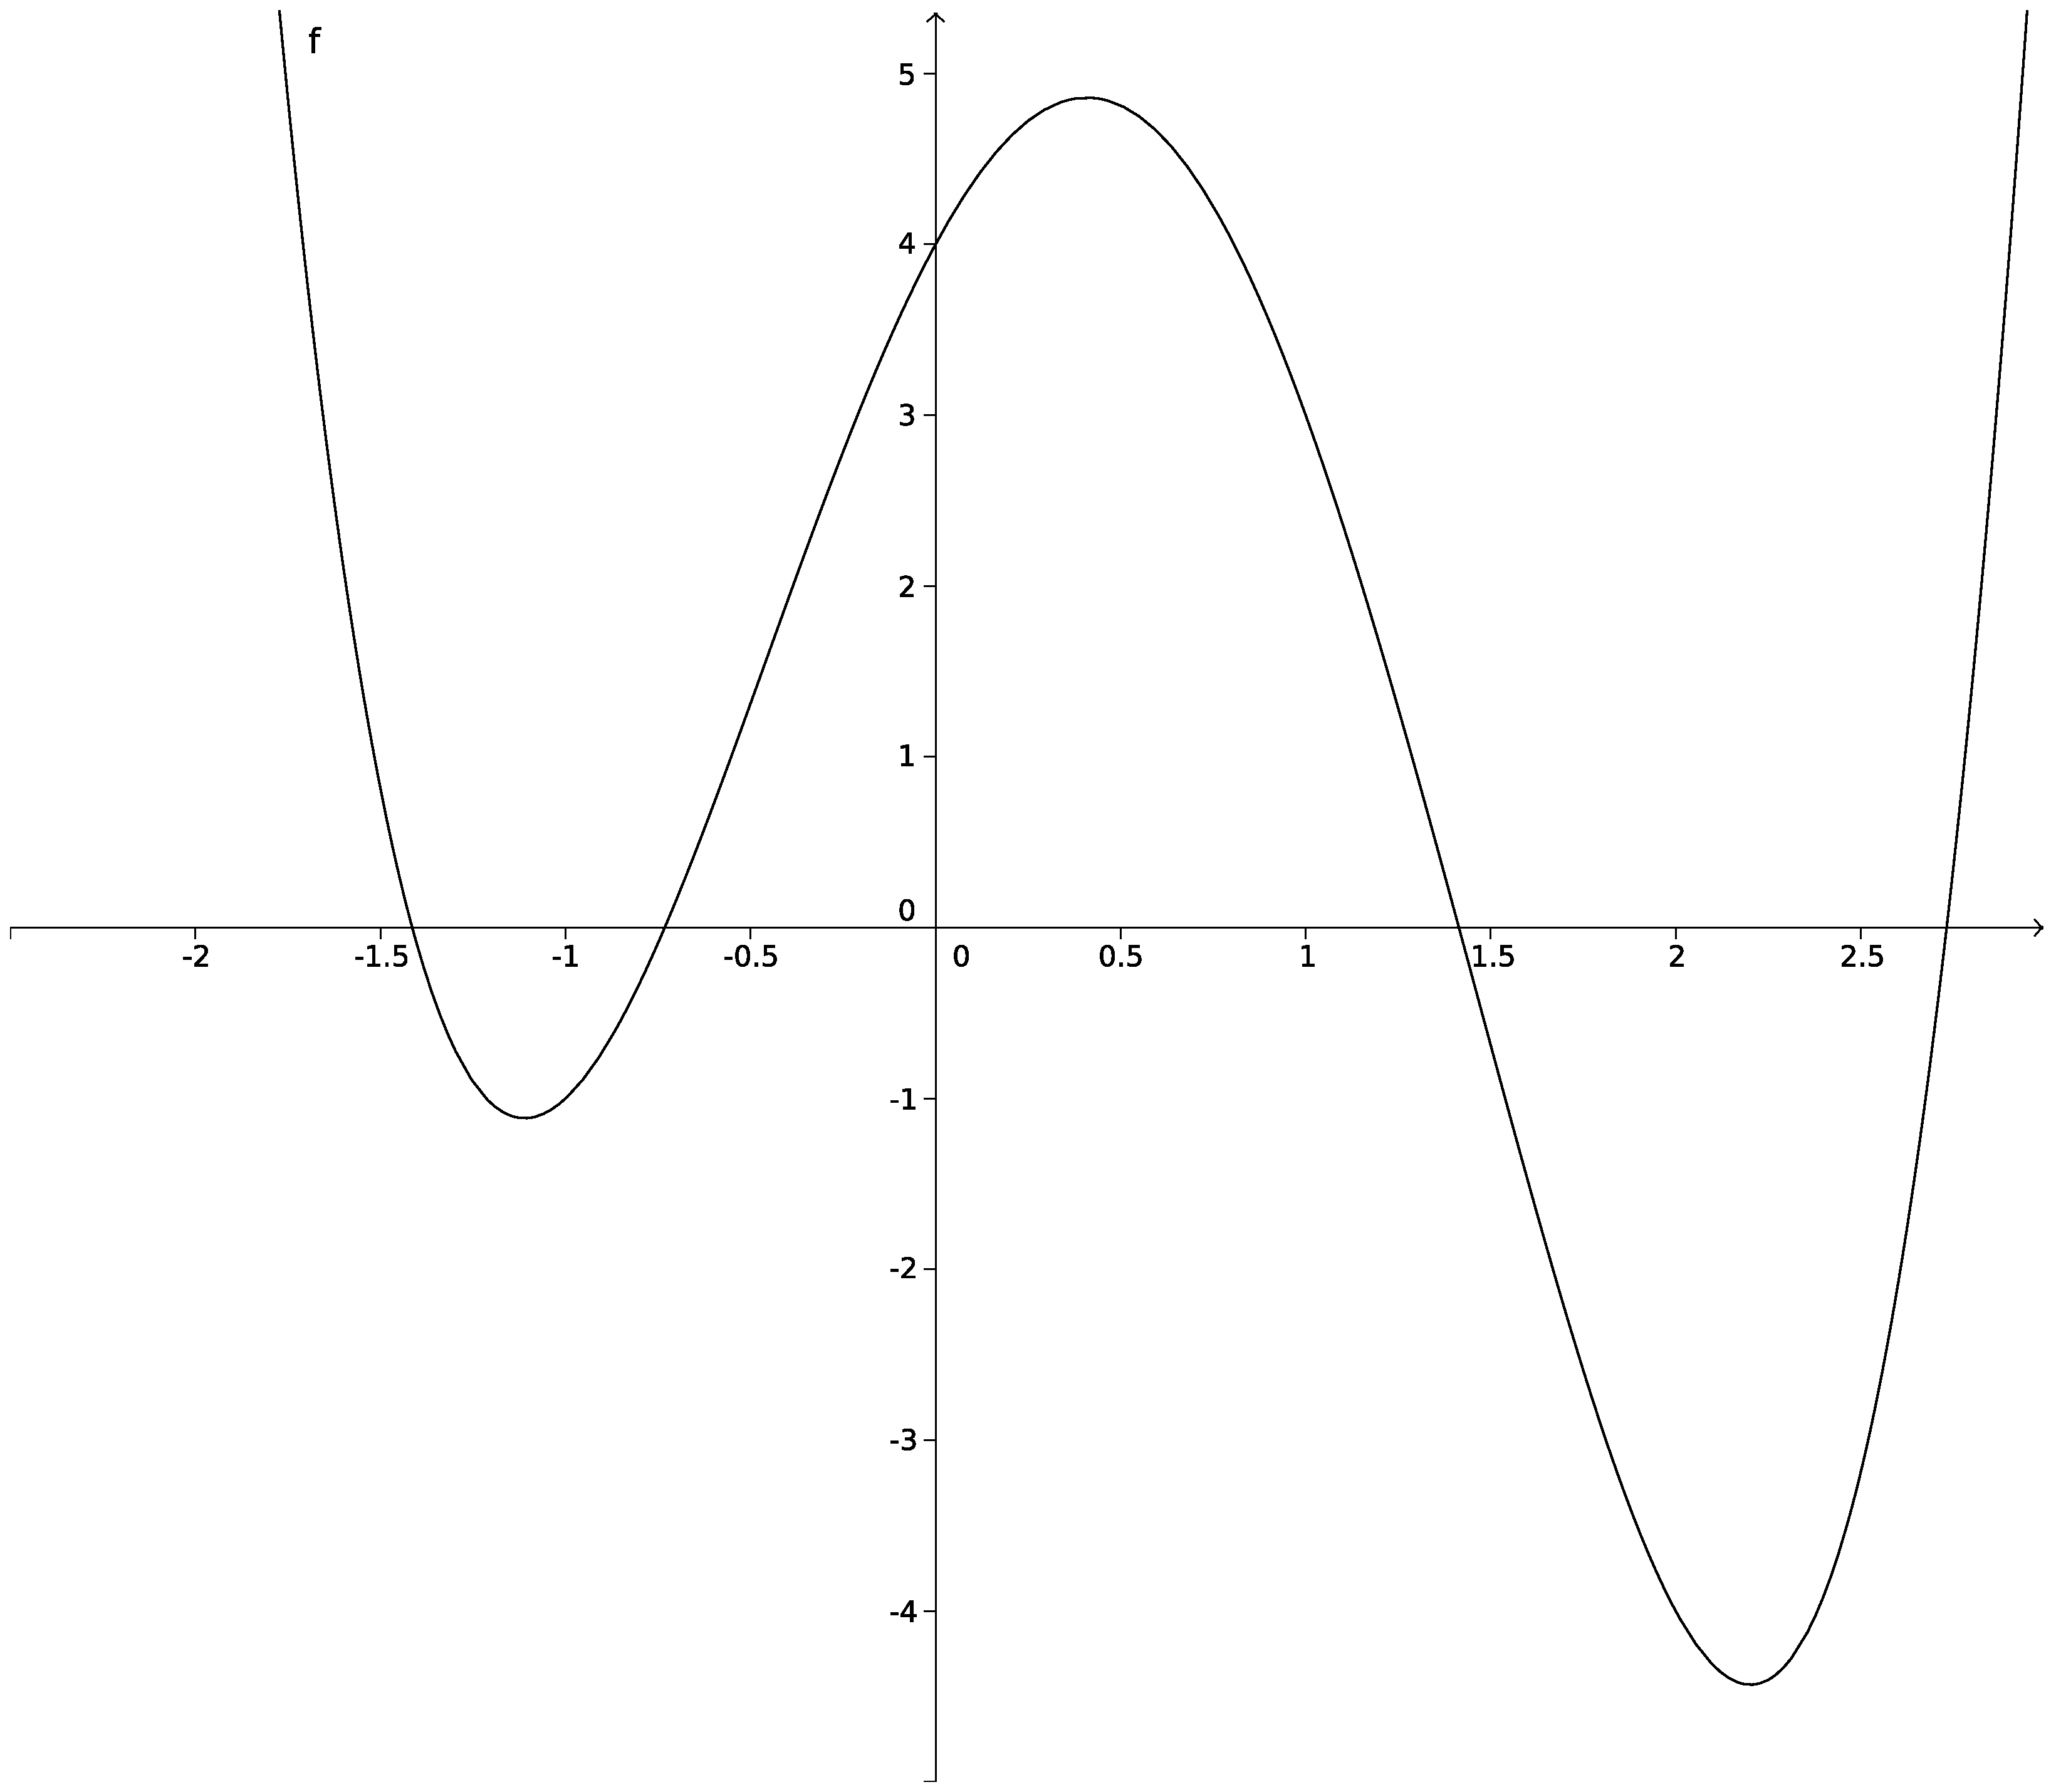
\includegraphics[scale=0.15]{./bisecc_f.eps}
    \end{center}
  \end{itemize}
\end{frame}
%%%%
\begin{frame}
  \frametitle{Ejemplo}
  \scriptsize{
  \begin{table}[!ht]
    \begin{center}
      \begin{tabular}{|c||c||c||c||c||c|}\hline
      $k$  & $a$ & $p$ & $b$ & $f(p)$ & $\frac{b-a}{2}$\\\hline\hline
      1 & -2.00000000 & -1.50000000 & -1.00000000 & 0.81250000 & 1.00000000 \\\hline 
    2 & -1.50000000 & -1.25000000 & -1.00000000 & -0.90234375 & 0.50000000 \\\hline
    3 & -1.50000000 & -1.37500000 & -1.25000000 & -0.28881836 & 0.25000000 \\\hline
    4 & -1.50000000 & -1.43750000 & -1.37500000 & 0.19532776 & 0.12500000 \\\hline
    5 & -1.43750000 & -1.40625000 & -1.37500000 & -0.06266689 & 0.06250000 \\\hline
    6 & -1.43750000 & -1.42187500 & -1.40625000 & 0.06226259 & 0.03125000 \\\hline
    7 & -1.42187500 & -1.41406250 & -1.40625000 & -0.00120812 & 0.01562500 \\\hline
    8 & -1.42187500 & -1.41796875 & -1.41406250 & 0.03027437 & 0.00781250 \\\hline
    9 & -1.41796875 & -1.41601562 & -1.41406250 & 0.01447008 & 0.00390625 \\\hline
    10 & -1.41601562 & -1.41503906 & -1.41406250 & 0.00661524 & 0.00195312 \\\hline
    11 & -1.41503906 & -1.41455078 & -1.41406250 & 0.00269963 & 0.00097656 \\\hline
    12 & -1.41455078 & -1.41430664 & -1.41406250 & 0.00074477 & 0.00048828 \\\hline
    13 & -1.41430664 & -1.41418457 & -1.41406250 & -0.00023192 & 0.00024414 \\\hline
    14 & -1.41430664 & -1.41424561 & -1.41418457 & 0.00025636 & 0.00012207 \\\hline
    15 & -1.41424561 & -1.41421509 & -1.41418457 & 0.00001220 & 0.00006104 \\\hline
    16 & -1.41421509 & -1.41419983 & -1.41418457 & -0.00010986 & 0.00003052 \\\hline
    17 & -1.41421509 & -1.41420746 & -1.41419983 & -0.00004883 & 0.00001526\\\hline
     \end{tabular}
     \caption{Resultados Bisecci\'on.}\end{center}
     \label{tab_bisecc}
    \end{table}}
\end{frame}
%%%%%%
\section{M\'etodo de Falsa Posici\'on o Regula Falsi.}
\begin{frame}[fragile]
  \frametitle{M\'etodo de Falsa Posici\'on o Regula Falsi.}
  \begin{itemize}
    \item El m\'etodo de la falsa posici\'on o Regula Falsi, es otra alternativa usada para resolver el problema de encontrar el
    cero de una funci\'on y difiere del m\'etodo de bisecci\'on en la forma como se consiguen los valores de $c_n$.
    \item<2-> Sea $f(a)f(b) < 0$ y sea la recta que une los puntos $(a, f (a))$, $(b, f (b))$ cuya pendiente es $m =
    \frac{f(b)-f(a)}{b-a}$,
    \item<3-> pero si $(c, 0)$ es el punto de intersecci\'on de la recta con el eje $x$, entonces tambi\'en $m = \frac{0 - f(b)}{c-b}$, obteniendo
    \begin{block}{}      
      $$
        c = \frac{af(b)-bf(a)}{f(b)-f(a)}
      $$
    \end{block}    
  \end{itemize}
\end{frame}
%%%%%%
\begin{frame}
  \frametitle{M\'etodo de Falsa Posici\'on o Regula Falsi.}
  \begin{center}
    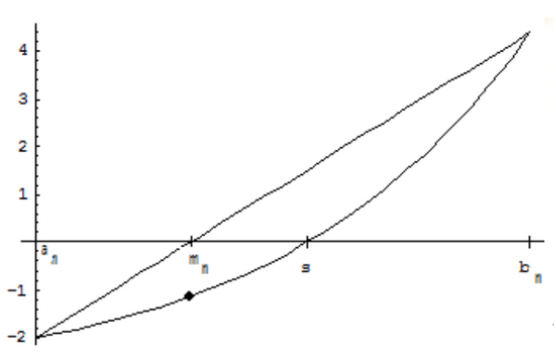
\includegraphics[scale=0.7]{regfalsi.png}
  \end{center}
\end{frame}
%%%%%%
\begin{frame}[fragile]
  \frametitle{M\'etodo de Falsa Posici\'on o Regula Falsi.}
  \begin{itemize}
    \item<1-> Al igual que para el m\'etodo de bisecci\'on se tienen tres posibilidades:
      \begin{itemize}
        \item[i)]<2-> $f (c) = 0$  
        \item[ii)]<3-> $f (a)f (c) < 0$ 
        \item[iii)]<4-> $f (c)f (b) < 0$.
      \end{itemize}
      \item<5-> Si $f (c) = 0$, entonces $c$ es un cero de $f$.
      \item<6-> Si $f (a)f (c) < 0$, entonces hay un cero de $f$ en $[a; c]$.
      \item<7-> Si $f (c)f (b) < 0$, entonces hay un cero de $f$ en $[c; b]$.
      \item<8-> Lo anterior sugiere un proceso iterativo que se concreta tomando
      \begin{block}{}
      $$
      c_n = \frac{a_nf(b_n)-b_nf(a_n)}{f(b_n)-f(a_n)} \quad\forall n=0,1,2,\ldots
      $$  
      \end{block}      
    \end{itemize}  
\end{frame}
%%%%%
\begin{frame}
  \frametitle{M\'etodo de Falsa Posici\'on o Regula Falsi.}
  \begin{block}{Teorema}    
      Sea $f$ dos veces continuamente diferenciable en $[a,b]$ con $\alpha$ una \'unica ra\'iz en $[a,b]$. Supongamos
     $f(a)f(b)<0$, $f'(\alpha) \neq 0$, y $f''$ no cambia de signo en $[a,b]$. Si $M = \left|\frac{\omega -
     \alpha}{2}\right| \max_{x \in [a,b]}\left|\frac{f''(x)}{f'(x)}\right|<1$ con $\omega=a$ o $\omega=b$ seg\'un sea el
     caso, entonces el m\'etodo de Regula Falsi converge. Esta convergencia es lineal.     
  \end{block}  
\end{frame}
%%%%%
\begin{frame}
  \frametitle{M\'etodo de Falsa Posici\'on o Regula Falsi.}
  \begin{block}{Demostraci\'on}
    \begin{itemize}      
      \item<1->Suponiendo $f''(x)>0$ en $[a,b]$, es decir, $f$ convexa. Entonces el segmento de recta que une $(x_1,f(x_1))$ y $(x_2,f(x_2))$ est\'a por encima de la gr\'afica de $f$, $\forall a\leq x_1 \leq x_2\leq b$. (Si
$f''<0$, cambiar $f$ por $-f$ y hacer el mismo razonamiento). 
\item<2->\textbf{Caso 1:} $f'(\alpha)>0$. Aqu\'i resulta que $c$ siempre verifica que $a<c<\alpha$. En este caso
$b-\alpha=constante$. Sea $a_n=n$-\'esimo valor de $a$ en el procedimiento y dado que
$$
c = b - f(b)\left[\frac{b-a}{f(b)-f(a)}\right]
$$    \end{itemize}
  \end{block}
\end{frame}
%%%%
\begin{frame}
   \frametitle{M\'etodo de Falsa Posici\'on o Regula Falsi.}
   \begin{itemize}
     \item<1->se tiene que 
     \scriptsize{
     \begin{eqnarray}
      \nonumber c - \alpha & = &  b - \alpha - f(b)\left[\frac{b-a}{f(b)-f(a)}\right] =
     \frac{(b-\alpha)(f(b)-f(a))-bf(b)+af(b)}{f(b)-f(a)}\\
     \nonumber & = & \frac{-\alpha f(b)+\alpha f(a)-bf(a)+af(b)}{f(b)-f(a)} =
     \frac{(a-\alpha)f(b)-(b-\alpha)f(a)}{f(b)-f(a)}\\
     \nonumber & = & (a-\alpha)(b-\alpha)\frac{1}{f(b)-f(a)}\left[\frac{f(b)}{b-\alpha}-\frac{f(a)}{a-\alpha}\right]\\
     \nonumber & = &
     \displaystyle(a-\alpha)(b-\alpha)\frac{1}{\displaystyle\frac{f(b)-f(a)}{b-a}}\frac{\left[\displaystyle\frac{f(b)}{
     b-\alpha} -\frac { f(a)}{ a-\alpha } \right]}{ b-a } \\
     \nonumber c - \alpha & = & \frac{1}{2}(a-\alpha)(b-\alpha)\frac{f''(\eta)}{f'(\xi)}, \quad \eta,\xi \in (a,b) 
     \end{eqnarray}
     }
    \end{itemize}
 \end{frame}
 %%%%
 \begin{frame}
    \frametitle{M\'etodo de Falsa Posici\'on o Regula Falsi.}
 \begin{itemize}
  \item<1-> Por lo tanto resulta que:    
     $$
     a_{n+1}-\alpha = \frac{1}{2}(a_n-\alpha)(b-\alpha)\frac{f''(\eta_n)}{f'(\xi_n)}, \quad \eta_n,\xi_n \in (a_n,b)
     $$    
  \item<2-> Se tiene as\'i que    
     $$
     |\xi_{n+1}| \leq M|\xi_n| \mbox{ con } M = \frac{b-\alpha}{2}\max_{x \in [a,b]}\left|\frac{f''(x)}{f'(x)}\right|
     $$
  \item<3-> Por lo tanto $|\xi_{n+1}| \leq M^n|\xi_0|$ y si $M<1$ se puede asegurar que $\lim \xi_n = 0$ y que la convergencia es
     lineal.
    \end{itemize}
 \end{frame}
 %%%%
 \begin{frame}
    \frametitle{M\'etodo de Falsa Posici\'on o Regula Falsi.}
    \begin{itemize}
      \item<1->\textbf{Caso 2:} En este caso $c$ siempre satisface
           $$
           \alpha < c < b
           $$
           y $\alpha -a=constante$. Se obtienen las mismas conclusiones que en el caso 1, pero con
           $$
           M = \left|\frac{a-\alpha}{2}\right|\max_{x \in [a,b]}\left|\frac{f''(x)}{f'(x)}\right|
           $$
    \end{itemize}
 \end{frame}
 %%%%
 \begin{frame}
    \frametitle{M\'etodo de Falsa Posici\'on o Regula Falsi.}
    \small{
\begin{algorithm}[H]
  \SetKwInOut{Input}{input}
  \SetKwInOut{Output}{output}
  \caption{Algoritmo de Regula Falsi.}
  \Input{$a,b \in \mathbb{R}$, N\'umero m\'aximo de iteraciones $N$, tolerancia $TOL$.}
  \Output{Soluci\'on aproximada $p$ tal que $f(p) \approx 0$.}
  $i \leftarrow 1$\\
  \While{$i \leq N$}
  {
   $\displaystyle p \leftarrow b - f(b)\left(\frac{b-a}{f(b)-f(a)}\right)$\\
   $i \leftarrow i +1$\\
   \If{$|f(p)|<TOL$}
   {
     Salida($p$); EXIT\\
   }
   \eIf{$f(a)f(p)>0$}
   {
      $a \leftarrow p$\\
   }
   {
     $b \leftarrow p$\\
   }
  }
  \label{RF_alg}
\end{algorithm}}
\end{frame}
%%%%
\begin{frame}
  \frametitle{M\'etodo de Falsa Posici\'on o Regula Falsi.}
  Los resultados obtenidos al aplicar el m\'etodo de falsa posici\'on al ejemplo presentado anteriormente son:
  \scriptsize{
  \begin{center}
  \begin{table}[!ht]
    \begin{center}
    \begin{tabular}{|c||c||c||c||c|}\hline
  $k$  & $a$ & $p$ & $b$ & $f(p)$ \\\hline\hline
  1 & -2.00000000 & -1.07692308 & -1.00000000 & -1.10374287 \\\hline
2 & -2.00000000 & -1.15467487 & -1.07692308 & -1.09517990 \\\hline
3 & -2.00000000 & -1.22537135 & -1.15467487 & -0.97314218 \\\hline
4 & -2.00000000 & -1.28347785 & -1.22537135 & -0.78093935 \\\hline
5 & -2.00000000 & -1.32725869 & -1.28347785 & -0.57596833 \\\hline
6 & -2.00000000 & -1.35806966 & -1.32725869 & -0.39853249 \\\hline
7 & -2.00000000 & -1.37870356 & -1.35806966 & -0.26363401 \\\hline
8 & -2.00000000 & -1.39205970 & -1.37870356 & -0.16922303 \\\hline
9 & -2.00000000 & -1.40051361 & -1.39205970 & -0.10652517 \\\hline
%10 & -2.00000000 & -1.40578848 & -1.40051361 & -0.06623504 \\\hline
%11 & -2.00000000 & -1.40905028 & -1.40578848 & -0.04086781 \\\hline
%12 & -2.00000000 & -1.41105602 & -1.40905028 & -0.02509622 \\\hline
%13 & -2.00000000 & -1.41228514 & -1.41105602 & -0.01536614 \\\hline
%14 & -2.00000000 & -1.41303675 & -1.41228514 & -0.00939167 \\\hline
%15 & -2.00000000 & -1.41349577 & -1.41303675 & -0.00573383 \\\hline
%16 & -2.00000000 & -1.41377588 & -1.41349577 & -0.00349829 \\\hline
%17 & -2.00000000 & -1.41394673 & -1.41377588 & -0.00213348 \\\hline
%18 & -2.00000000 & -1.41405091 & -1.41394673 & -0.00130081 \\\hline
%19 & -2.00000000 & -1.41411442 & -1.41405091 & -0.00079300 \\\hline
%20 & -2.00000000 & -1.41415313 & -1.41411442 & -0.00048339 \\\hline
%21 & -2.00000000 & -1.41417673 & -1.41415313 & -0.00029464 \\\hline
%22 & -2.00000000 & -1.41419111 & -1.41417673 & -0.00017958 \\\hline
%23 & -2.00000000 & -1.41419988 & -1.41419111 & -0.00010946 \\\hline
\vdots & \vdots & \vdots & \vdots & \vdots \\\hline
24 & -2.00000000 & -1.41420522 & -1.41419988 & -0.00006671 \\\hline
25 & -2.00000000 & -1.41420848 & -1.41420522 & -0.00004066 \\\hline
26 & -2.00000000 & -1.41421046 & -1.41420848 & -0.00002478 \\\hline
27 & -2.00000000 & -1.41421167 & -1.41421046 & -0.00001510 \\\hline
28 & -2.00000000 & -1.41421241 & -1.41421167 & -0.00000921 \\\hline
 \end{tabular}
 \caption{Resultados Regula Falsi.}\end{center}
 \label{tab_regfalsi}
\end{table}
  \end{center}}
\end{frame}
%%%%
\section{M\'etodo de Illinois}
\begin{frame}
  \frametitle{M\'etodo de Illinois}
  \begin{itemize}
    \item<1-> La intenci\'on del m\'etodo es solucionar el problema de los extremos fijos que puede
    ocurrir en Regula Falsi. 
    \item<2->Este nuevo m\'etodo sigue el mismo procedimiento
    de la Regula Falsi.
    \item<3-> El nuevo punto $x_{i+1}$ se forma obteniendo la ra\'iz
    buscada $x^* \in (x_i ;x_{i+1})$. 
    \item<4->En primer lugar se emplea Regula Falsi, es decir,
    $$
      x_{i+1} = \frac{x_if_{i-1}-x_{i-1}f_i}{f_{i-1}-f_i}
    $$  
    donde se ha usado la notaci\'on
    $$
      f_i = f(x_i);\quad \forall i;
    $$
  \end{itemize}
\end{frame}
%%%%
\begin{frame}
  \frametitle{M\'etodo de Illinois}
  \begin{itemize}
    \item<1-> A continuación
    \begin{enumerate}
      \item[i)] si $f_i\cdot f_{i+1} < 0$ entonces $(x_{i-1}; f_{i-1})$ se reemplaza por $(x_i ; f_i )$ y $x^* \in (x_i ;x_{i+1})$.
      \item[ii)] si $f_i\cdot f_{i+1} > 0$ entonces $(x_{i-1}; f_{i-1})$ se reemplaza por $(x_{i-1}; f_{i-1}/2)$ y $x^* \in (x_{i-1};x_{i+1})$.
    \end{enumerate}
    \item<2-> De esta manera cuando se est\'a en la situación ii), se calcula el siguiente punto de manera similar pero atendiendo a una f\'ormula ligeramente
    modificada
    \begin{block}{}
    $$
      x_{i+2} = \frac{x_{i+1}\frac{f_{i-1}}{2}-x_{i-1}f_{i+1}}{\frac{f_{i-1}}{2}-f_{i+1}}
    $$  
    \end{block}    
  \end{itemize}    
\end{frame}
%%%%
\begin{frame}
  \frametitle{M\'etodo de Illinois}
  \begin{center}
    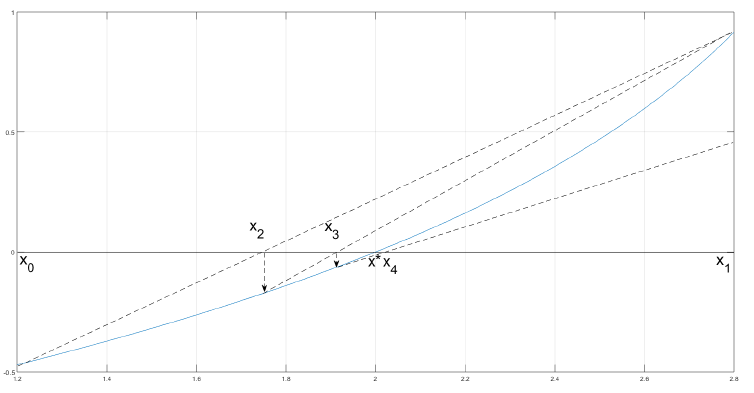
\includegraphics[scale=0.5]{MetIllinois.png}
  \end{center}
\end{frame}
\begin{frame}
  \frametitle{Algoritmo del M\'etodo de Illinois}
  \small{ 
  \begin{algorithm}[H]
    \SetAlgoLined
    \KwData{Un intervalo $[a,b]$ tal que $f(a)\cdot f(b) < 0$}
    \KwResult{Una aproximaci\'on $x$ a la ra\'iz de $f(x)$}
    $i \leftarrow 1$; $x_{i-1} \leftarrow a$\;
    $f_{i-1} \leftarrow f(a)$; $x_{i} \leftarrow b$\;
    $f_{i} \leftarrow f(b)$\;
    \While{ $|f_i| > \epsilon$ }{
      $x_{i+1} \leftarrow \frac{x_if_{i-1}-x_{i-1}f_i}{f_{i-1}-f_i}$; $f_{i+1} \leftarrow f(x_{i+1})$\;
      \If{ $f_{i+1}\cdot f_{i} < 0$ }{
        $(x_{i-1}; f_{i-1}) \leftarrow (x_{i}; f_{i})$\;
      }
      \Else{
        $(x_{i-1}; f_{i-1}) \leftarrow (x_{i-1}; f_{i-1}/2)$\;
      }
      $i \leftarrow i+1$\;
    }
    \KwRet $x_i$
  \end{algorithm}}
\end{frame}
%%%%%
%%%%
\begin{frame}
  \frametitle{M\'etodo de Illinois.}
  Los resultados obtenidos al aplicar el m\'etodo de Illinois al ejemplo presentado anteriormente son:    \begin{center}
  \begin{table}[!ht]
    \begin{center}
    \begin{tabular}{|c||c||c||c||c|}\hline
  $k$  & $a$ & $p$ & $b$ & $|f(p)|$ \\\hline\hline
  1 & -2.00000000 & -1.07692307 & -1.07692307 & 1.10374286e+00\\\hline
  2 & -2.00000000 & -1.22034600 & -1.22034600 & 9.85725880e-01\\\hline
  3 & -2.00000000 & -1.41316536 & -1.41316536 & 8.36748888e-03\\\hline
  4 & -1.41316536 & -1.41642075 & -1.41642075 & 1.77379628e-02\\\hline
  5 & -1.41642075 & -1.41420880 & -1.41420880 & 3.80691452e-05\\\hline
  6 & -1.41642075 & -1.41421354 & -1.41421354 & 1.72544154-07\\\hline
 \end{tabular}
 \caption{Resultados Illinois.}\end{center}
 \label{tab_illinois}
\end{table}
  \end{center}
\end{frame}
%%%%
\section{M\'etodos de Punto Fijo}
\begin{frame}
  \frametitle{M\'etodos de Punto Fijo}
  \begin{itemize}
    \item<1-> El m\'etodo de aproximaciones sucesivas (o de punto fijo) 
    para determinar una soluci\'on de la ecuaci\'on no lineal $f(x)=0$
    se basa en el teorema del punto fijo. 
    \item<2-> Para ello el primer paso que se realiza en este m\'etodo consiste
    en reescribir la ecuaci\'on $f(x)=0$ en la forma $x = g(x)$.
    \item<3-> Una vez hecho esto, se escoge alg\'un $x_0$ como aproximaci\'on inicial al punto fijo
    $x^*$, y se genera una sucesi\'on de aproximaciones mediante las iteraciones:
    \begin{block}{}
        $$
        x_{n+1} = g(x_n), \qquad n=0,1,2,\ldots
        $$
    \end{block}
    donde se espera que la sucesi\'on $\{x_n\}$ converja al punto fijo $x^*$.
  \end{itemize}
\end{frame}
%%%%%
\begin{frame}
  \frametitle{M\'etodos de Punto Fijo}
  \begin{block}{Proposici\'on}
    Si $f$ es una funci\'on continua y $x_n$ converge, entonces su l\'imite $x^*$ es un punto fijo de $f$.
  \end{block}
  \uncover<2->{La prueba de la proposici\'on es la siguiente cadena de igualdades
  $$
  f(x^*) = \lim_n f(x_n) = \lim_n x_n = \lim_n x_{n+1} = x^*
  $$
  }
\end{frame}
%%%%
\begin{frame}
  \frametitle{M\'etodos de Punto Fijo}
  \begin{itemize}
    \item<1-> Existen m\'ultiples posibilidades para transformar la ecuaci\'on $f(x) = 0$ en otra del tipo $x =
    g(x)$.
    \item<2-> Por ejemplo podr\'ia despejarse (de la forma que sea) $x$ de la expresi\'on de la ecuaci\'on $f (x) = 0$.
    \item<3-> O podr\'ia sumarse la variable $x$ en ambos lados de la ecuaci\'on y designar por $g(x)$ a $(f (x) + x)$:
    $$
      0 = f(x) \Leftrightarrow x = f(x) + x = g(x)
    $$
  \end{itemize}
\end{frame}
%%%%
\begin{frame}
  \frametitle{M\'etodos de Punto Fijo}
\begin{figure}[ht]
\centering
\subfigure[Proceso divergente (Escalera).]{
	%\rule{4cm}{3cm}   
	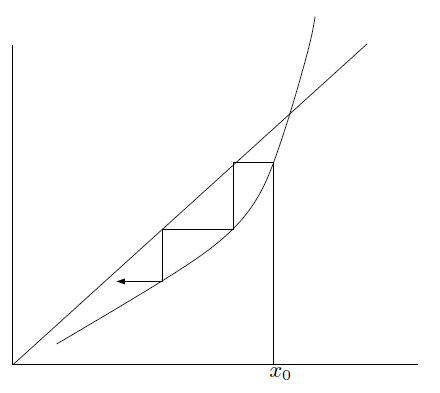
\includegraphics[scale=0.35]{diver.png}
	\label{PF_div}
}
\subfigure[Proceso convergente (Escalera).]{
	%\rule{4cm}{3cm}
	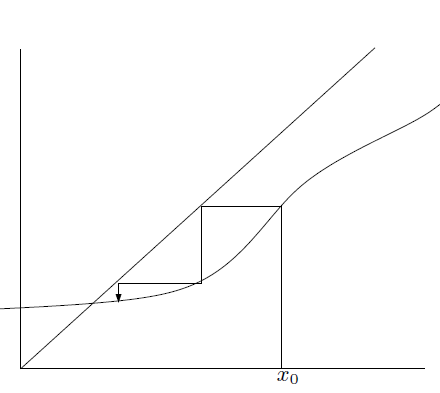
\includegraphics[scale=0.35]{conver.png}
	\label{PF_conv}
}
\caption{Proceso de Punto Fijo.}
\end{figure}
\end{frame}
%%%%
\begin{frame}
  \frametitle{M\'etodos de Punto Fijo}
  \begin{figure}[ht]
  \centering
  \subfigure[Proceso divergente (Oscilante).]{
    %\rule{4cm}{3cm}
    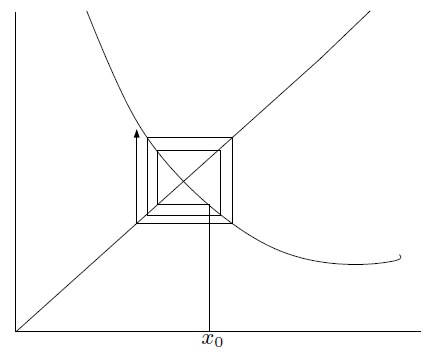
\includegraphics[scale=0.35]{diver2.png}
    \label{PF_div2}
  }
  \subfigure[Proceso convergente (Oscilante).]{
    %\rule{4cm}{3cm}
    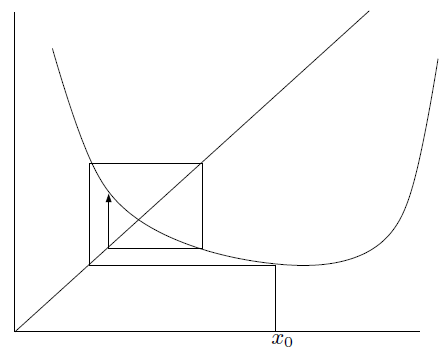
\includegraphics[scale=0.35]{conver2.png}
    \label{PF_conv2}
  }
  \caption{Proceso de Punto Fijo.}
  \end{figure}
\end{frame}
%%%%%
\begin{frame}
  \frametitle{M\'etodos de Punto Fijo}
  \begin{itemize}
    \item Hallar num\'ericamente una de las ra\'ices de $f(x) = x^2 -x-2 = 0$. Sus ra\'ices exactas son $x_1 = -1$ y $x_2 = 2$.
     Hallando \'unicamente en el c\'alculo de la ra\'iz $x^* = 2$ tomando como punto de partida $x_0=2.1$ y definiendo $g$ como.
     \begin{itemize}
      \item $g_1(x) = x^2-2$
      \item $g_2(x) = \sqrt{x+2}$
      \item $g_3(x) = 1+\dfrac{2}{x}$
      \item $g_4(x) = \dfrac{x^2+2}{2x-1}$
     \end{itemize}
  \end{itemize}
\end{frame}
%%%%%
\begin{frame}
  \frametitle{M\'etodos de Punto Fijo}
  \begin{center}
    \small{
    \begin{tabular}{|c|c|c|c|c|}\hline
    k & $g_1(x)$ & $g_2(x)$ & $g_3(x)$ & $g_4(x)$ \\\hline\hline 
    1 & 2.41000000e+00 & 2.02484567 & 1.95238095 & 2.00312500\\\hline
    2 & 3.80810000e+00 & 2.00620180 & 2.02439024 & 2.00003248\\\hline
    3 & 1.25016256e+01 & 2.00154985 & 1.98795180 & 2.00000000 \\\hline
    4 & 1.54290642e+02 & 2.00038742 & 2.00606060 & \\\hline
    5 & 2.38036024e+04 & 2.00009685 & 1.99697885 & \\\hline
    6 & 5.66611489e+08 & 2.00002421 & 2.00151285 & \\\hline
    7 & 3.21048579e+17 & 2.00000605 & 1.99924414 & \\\hline
    8 & 1.03072190e+35 & 2.00000151 & 2.00037807 & \\\hline
    9 & 1.06238764e+70 & & 1.99981099 & \\\hline
    10 & 1.12866751e+140 & & 2.00009450 & \\\hline
    11 & 1.27389035e+280 & & 1.99995274 & \\\hline
    12 & & & 2.00002362 & \\\hline
    13 & & & 1.99998818 & \\\hline
    14 & & & 2.00000590 & \\\hline
    15 & & & 1.99999704 & \\\hline
    \end{tabular}}
  \end{center}
\end{frame}
%%%%%
\begin{frame}
  \frametitle{M\'etodos de Punto Fijo}
  \begin{block}{Definici\'on:}
    Una aplicaci\'on $T : X \to X$ con $X \subseteq \mathbb{R}^n$ se denomina contracci\'on sobre $X$ si existe un n\'umero
real $K$, con $0 < K < 1$, tal que para todo $x, y \in X$
$$
\|Tx - Ty\| \leq K \|x - y\|
$$
en alguna norma vectorial $\|\cdot\|$.
  \end{block}
\end{frame}
%%%%%ç
\begin{frame}
  \frametitle{M\'etodos de Punto Fijo}
  \begin{itemize}
    \item<1-> Geom\'etricamente esto significa que dos puntos cualesquiera $x, y \in X$ tienen im\'agenes m\'as cercanas que ellos
    mismos.
    \item<2-> De ah\'i el nombre de contracci\'on para la aplicaci\'on $T$.    
    \item<3-> \textbf{Ejemplo:} La funci\'on $g: [1, 3] \to [1, 3]$ definida por $g(x) = \sqrt{x + 2}$ es una contracci\'on
    en $X = [1, 3]$.
    \item<4->Primero verificando que $g(x) \in [1, 3]$ si $x \in [1, 3]$:
    $$
    x \in [1,3] \Leftrightarrow 1 \leq x \leq 3 \Leftrightarrow 3 \leq x+2 \leq 5  \Leftrightarrow \sqrt{3} \leq
    \sqrt{x+2} \leq \sqrt{5}
    $$
    
    Por lo tanto, $g(x) = \sqrt{x + 2} \in [1, 3]$.
  \end{itemize}
\end{frame}
%%%%%
\begin{frame}
  \frametitle{M\'etodos de Punto Fijo}
  \begin{itemize}
    \item<1-> Por otro lado, por el teorema del valor medio
    $$
    |g(x)-g(y)|= |g'(\eta)||x-y| \quad\mbox{con $\eta$ entre $x$ y $y$}
    $$
    y debido a que
    $$
    g'(x) = \frac{1}{2\sqrt{x+2}}  \Rightarrow \max_{x\in[1,3]}|g'(x)|=g'(1)= \frac{1}{2\sqrt{3}}
    $$
    \item<2->Por lo tanto
    $$
    |g(x)-g(y)| \leq \frac{1}{2\sqrt{3}}|x-y|
    $$
    Se concluye que $g$ es una contracci\'on con $K = \frac{1}{2\sqrt{3}}<1$.
  \end{itemize}
\end{frame}
%%%%%
\begin{frame}
  \frametitle{M\'etodos de Punto Fijo}
  \begin{block}{Teorema de punto fijo de Banach}
    Si $X$ es un conjunto cerrado conexo de $\mathbb{R}^n$ y $T$ es una
contracci\'on sobre $X$, entonces $T$ tiene un \'unico punto fijo en $X$, y dado cualquier punto de comienzo $x_0 \in X$,
la sucesi\'on generada por iteraci\'on de punto fijo
$$
x_{n+1} = Tx_n, \quad n=0,1,2,\ldots
$$
converger\'a al punto fijo $x^*$ de $T$.
  \end{block}
\end{frame}
%%%%%
\begin{frame}
  \frametitle{M\'etodos de Punto Fijo}
  \begin{block}{Demostraci\'on:}
    Sea $x_0 \in X$, y sea $\{x_n\}$ la sucesi\'on generada. Para cada $m \in
    \mathbb{N}$, $x_{m+1} - x_m = T x_m - T x_{m-1}$, y por ser $T$ una contracci\'on:
    $$
    \|x_{m+1} - x_m\| = \|T x_m - T x_{m-1}\| \leq K\|x_m - x_{m-1}\|
    $$
    con $0 < K < 1$. Procediendo recursivamente, se obtiene
    $$
    \|x_{m+1} - x_m\| \leq K^m\|x_1 - x_0\| \quad \forall m \in \mathbb{N}  
    $$
  \end{block}
\end{frame}
%%%%
\begin{frame}
  \frametitle{M\'etodos de Punto Fijo}
  \begin{block}{Demostraci\'on:}
    Utilizando este resultado para toda $n > m$ se obtiene

\begin{eqnarray}
 \nonumber & & \|x_n - x_m\|  =   \|x_n - x_{n-1} + x_{n-1} - x_{n-2} + \cdots + x_{m+1} - x_m\|\\
 \nonumber & & \leq \|x_n - x_{n-1}\| + \|x_{n-1} - x_{n-2}\| + \cdots + \|x_{m+1} - x_m\|\\
 \nonumber & & \leq (K^{n-1} + K^{n-2} + \cdots + K^m)\|x_1 - x_0\|\\
 \nonumber & & \leq K^m(1 + K + K^2 + \cdots + K^{n-m-1})\|x_1 - x_0\|\\
 \nonumber & & \leq K^m\frac{1-K^{n-m}}{1-K}\|x_1 - x_0\|
\end{eqnarray}
y como $0 < K^{n-m} < 1$, entonces
$$
\|x_n - x_m\| \leq K^m\frac{1}{1-K}\|x_1 - x_0\|
$$
\end{block}
\end{frame}
%%%%
\begin{frame}
  \frametitle{M\'etodos de Punto Fijo}
  \begin{block}{Demostraci\'on:}
    Por lo tanto
$$
\lim_{n,m \to \infty} \|x_n - x_m\| \leq \lim_{m \to \infty}K^m\frac{1}{1-K}\|x_1 - x_0\|=0
$$
lo cual implica que la sucesi\'on $\{x_n\}$ generada es una sucesi\'on de Cauchy. Como $T$ est\'a
definida sobre el conjunto cerrado $X$ la sucesi\'on de Cauchy $\{x_n\}$ tiene un l\'imite $x^* \in X$:
$$
x^* = \lim_{n \to \infty}x_n
$$
\end{block}
\end{frame}
%%%%
\begin{frame}
  \frametitle{M\'etodos de Punto Fijo}
  \begin{block}{Demostraci\'on:}
Este l\'imite $x^* \in X$ es un punto fijo de $T$ pues
\begin{eqnarray}
\nonumber  \|x^* - T x^*\| & = & \|x^* - x_n + x_n - T x^*\| \\
\nonumber & \leq & \|x^* - x_n\| + \|x_n - T x^*\| \\
\nonumber & = & \|x^* - x_n\| + \|T x_{n-1} - Tx^*\|
\end{eqnarray}
implica que
$$
  \|x^* - Tx^*\| \leq  \|x^* - x_n\| + K \|x_{n-1} - x^*\| \to 0,\mbox{ cuando } n \to \infty.
$$
\end{block}
\end{frame}
%%%%
\begin{frame}
  \frametitle{M\'etodos de Punto Fijo}
  \begin{block}{Demostraci\'on:}
    Por lo tanto, $x^* = T x^*$. Adem\'as este es el \'unico punto fijo de $T$ en $X$, pues si hubiese otro, digamos $\eta$,
entonces
$$
\|x^* - \eta\| = \|Tx^* - T\eta\| \leq K \|x^* - \eta\| < \|x^* - \eta\|,
$$
lo cual no es posible. Por tanto, $x^*$ es el \'unico punto fijo de $T$ en $X$.
  \end{block}
\end{frame} 
%%%%%
\begin{frame}
  \frametitle{M\'etodos de Punto Fijo}  
    \begin{itemize}
      \item<1-> En resumen, para que una aplicaci\'on sea una buena funci\'on de iteraci\'on y produzca una sucesi\'on convergente al
      punto fijo basta con que ella sea una contracci\'on en un conjunto cerrado $X$ que contenga al punto fijo.
      \item<2-> Si $g$ es una funci\'on suave (tiene derivada continua en $X$), y si adem\'as
      $$
      \|g'(x)\| \leq K, \forall x \in X \mbox{ con } 0 < K < 1 ,
      $$
      entonces $g$ es una contracci\'on en $X$ con $K = \max_{x \in X} \|g'(x)\| < 1$. En efecto, para $x, y, \in X$,
      por el teorema del valor medio, se tiene
      $$
      \|g(x) - g(y)\| \leq \|g'(\eta)\|\|x - y\| \mbox{ con $\eta$ entre los puntos $x, y$}.
      $$
      \item<3-> Por lo tanto
      $$
      \|g(x) - g(y)\| \leq K \|x - y\| \mbox{ con } K = \max_{x \in X} \|g'(x)\| < 1.
      $$      
    \end{itemize}  
\end{frame}
%%%%
\begin{frame}
  \frametitle{Cota del error para el M\'etodo de Punto Fijo}
    \begin{itemize}
      \item<1-> La desigualdad
      $$
      \|x_n - x_m\| \leq K^m\frac{1}{1-K}\|x_1 - x_0\|
      $$
      es v\'alida para toda $n > m$. 
      \item<2-> Cuando $n \to \infty$, $x_n \to x^*$, y por
      tanto
      $$
      \|x_m - x^*\| \leq K^m\frac{1}{1-K}\|x_1 - x_0\| \quad \forall m \in \mathbb{N}
      $$
      \item<3-> Esta desigualdad, sirve para estimar el
      n\'umero de iteraciones necesarias para alcanzar una precisi\'on determinada en el c\'alculo del punto fijo $x^*$:
      $$
      n \geq \frac{\ln\left(\displaystyle\frac{\|x_n-x^*\|}{\|x_1-x_0\|}(1-K)\right)}{\ln(K)}
      $$      
    \end{itemize}
\end{frame}
%%%%
\begin{frame}
  \frametitle{Orden de Convergencia}
  \begin{block}{Teorema}
    Sea $f (x) = 0$ una ecuaci\'on no lineal y $x = g(x)$ su correspondiente ecuaci\'on de punto fijo. Bajo las siguientes
condiciones:
\begin{enumerate}
 \item $g$ es una contracci\'on sobre $X$.
 \item $g \in \mathcal{C}^1(X)$ ($g$ y $g'$ son continuas en $X$).
 \item $g$ es estrictamente mon\'otona sobre $X$ ($g'(x) \neq 0 , \forall x  \in X$).
\end{enumerate}
se tiene que
$$
\mbox{Si } x_0 \neq x^*, \mbox{ entonces } x_n \neq x^* , \forall n \in \mathbb{N},
$$
es decir, el proceso iterativo no puede terminar en un n\'umero finito de pasos.
  \end{block}
\end{frame}
\begin{frame}
  \frametitle{Orden de Convergencia}
  \begin{block}{Demostraci\'on:}
    Una demostraci\'on de este hecho se obtiene suponiendo lo contrario, es decir que $g(x_n ) =
x_n$ para alg\'un $n$. Si $n$ es el primer \'indice para el cual esto ocurre, entonces
$$
x_n = g(x_{n-1} ) \mbox{ y } x_n = g(x_n ) \mbox{ con } x_{n-1} \neq x_n.
$$
Luego, por el teorema del valor medio
$$
0 = g(x_n ) - g(x_{n-1}) = g'(\eta)(x_n - x_{n-1}) \mbox{ con $\eta$ entre $x_{n-1}$ y $x_n$},
$$
y debe tenerse $g'(\eta) = 0$ con $\eta \in X$, lo cual contradice la hip\'otesis de que $g'(x) \neq 0\quad \forall x \in X$.
  \end{block}
\end{frame}
%%%%
\begin{frame}
  \frametitle{Comportamiento asint\'otico del error}
  \begin{itemize}
    \item<1-> Se puede analizar como se comporta el error en el m\'etodo iterativo de punto fijo al
ir aumentando $n$:
$$
e_{n+1} = x_{n+1} - x^* = g(x_n) - g(x^*) = g'(\eta_n )(x_n - x^*) = g'(\eta_n)e_n .
$$
\item<2->Es decir:
$$
e_{n+1} = g'(\eta_n )e_n \mbox{ con $\eta_n$ entre $x_n$ y $x^*$} .
$$
\item<3-> Como $\eta_n$ est\'a entre $x_n$ y $x^*$ para cada $n$, y $x^*$ es el l\'imite de $x_n$, necesariamente se tiene que
$$
\lim_{n \to \infty}\eta_n = x^*
$$
  \end{itemize}
\end{frame}
%%%%%%
\begin{frame}
  \frametitle{Comportamiento asint\'otico del error}
  \begin{itemize}
    \item<1->Adem\'as $\displaystyle\lim_{n \to \infty}g'(\eta_n) = g'(x^*)$
    por ser $g'(x)$ continua. As\'i que
    $$
    e_{n+1} = g'(\eta_n )e_n = (g'(x^*) +\varepsilon_n)e_n
    $$
    donde $\varepsilon_n \to 0$ cuando $n \to \infty$.
    \item<2->Luego
    $$
    \lim_{n \to \infty}\frac{e_{n+1}}{e_n} = g'(x^*) +\lim_{n \to \infty}\varepsilon_n = g'(x^*)
    $$    
    \item<3-> Para valores suficientemente grandes de $n$ se tendr\'a que
    $$
    e_{n+1} \approx g'(x^*)e_n
    $$    
    \item<4->El error en la iteraci\'on $n + 1$ depende linealmente del error
    en la iteraci\'on $n$. Se puede decir que la sucesi\'on $\{x_n\}$ converge linealmente a $x^*$, y que el
    m\'etodo de punto fijo es un m\'etodo con orden de convergencia lineal o de orden uno.
  \end{itemize}
\end{frame}    
%%%%%
\begin{frame}
  \frametitle{Algoritmo de Punto Fijo}
  \begin{algorithm}[H]
    \SetKwInOut{Input}{input}
    \SetKwInOut{Output}{output}
    \caption{Algoritmo de Punto Fijo.}
    \Input{$x_0 \in \mathbb{R}$, N\'umero m\'aximo de iteraciones $N$, tolerancia $TOL$.}
    \Output{Soluci\'on aproximada $p$ tal que $g(p) = p$ satistace $f(p)\approx 0$.}
    $i \leftarrow 1$\\
    \While{$i \leq N$}
    {
     $\displaystyle p \leftarrow g(x_0)$\\
     $i \leftarrow i +1$\\
     \If{$|p-x_0|<TOL$}
     {
       Salida($p$), \quad    EXIT\\
     }
     
     $x_0  \leftarrow p$\\
    }
    \label{PF_alg}
   \end{algorithm}
\end{frame}
%%%%%
\section{M\'etodo de Newton-Raphson}
\begin{frame}
  \frametitle{M\'etodo de Newton-Raphson}
  \begin{itemize}
    \item<1-> Sea $f \in C^2 ([a, b])$ con $\alpha$ ra\'iz de $f$ en $[a,b]$ y $x_0$ un punto pr\'oximo a $\alpha$. Usando el desarrollo de Taylor de orden 1 de la funci\'on $f$ en torno a $x_0$, se tiene
    \begin{block}{}
    $$
      f(x) = f(x_0) + f'(x_0)(x-x_0) + \frac{1}{2}f''(\mu)(x-x_0)^2
    $$  
    \end{block}
    donde $\mu$ est\'a entre $x$ y $x_0$.
    \item<2-> Si $x_0$ est\'a cerca de $\alpha$ y $|f''(x_0)|$ no es demasiado grande, entonces la funci\'on
    \begin{block}{}
      $$
    \bar f(x) = f(x_0) + f'(x_0)(x-x_0)
    $$      
    \end{block}
    es una aproximaci\'on de $f(x)$ en una vecindad de $\alpha$. $\bar f(x)$ es una linealizaci\'on de $f(x)$ en el punto $(x_0 , f(x_0))$.
  \end{itemize}
\end{frame}
%%%%%
\begin{frame}
  \frametitle{M\'etodo de Newton-Raphson}
  \begin{itemize}
    \item<1-> Si en esta expresi\'on se despeja $x$ obtenemos una aproximaci\'on de $\alpha$ m\'as exacta de lo que era la estimaci\'on inicial $x_0$ . As\'i tenemos
    \begin{block}{}
    $$
    x = x_0 - \frac{f(x_0)}{f'(x_0)}, \textrm{ si } f(\alpha) = 0
    $$
    \end{block}
    \item<2-> Esto permite generar una sucesi\'on de aproximaciones de $\alpha$ a partir de la iteraci\'on de Newton-Raphson:
    \begin{block}{}
    $$
    x_{n+1} = x_n - \frac{f(x_n)}{f'(x_n)}, \quad n=0,1,2,\ldots
    $$    
    \end{block}
    \item<3-> En general se define la iteraci\'on de Newton-Raphson como 
    \end{itemize}
\end{frame}
%%%%%
%%%%%
\begin{frame}
  \frametitle{Interpretaci\'on Geom\'etrica}
  \begin{itemize}
    \item<1-> El m\'etodo de Newton tiene una interpretaci\'on geom\'etrica muy sencilla. Dada la ecuaci\'on $f(x) = 0$ en una
    variable, suponiendo conocido la aproximaci\'on $x_n$ a la ra\'iz $x^*$, $x_{n+1}$ se calcula como
    $$
    x_{n+1} = x_n - \frac{f(x_n)}{f'(x_n)}
    $$
    
    \item<2->es decir
    $$
    f(x_n) + (x_{n+1} - x_n)f'(x_n) = 0
    $$    
  \end{itemize}
\end{frame}
%%%%
\begin{frame}
  \frametitle{Interpretaci\'on Geom\'etrica}
  \begin{itemize}
    \item<1-> Si se reemplaza $x_{n+1}$ por la variable $x$, se obtiene la funci\'on $y = f(x_n) + f (x_n)(x - x_n)$, la cual tiene
    como gr\'afica a la recta tangente a $f(x)$ en el punto $(x_n , f (x_n))$.
    \item<2-> As\'i que $x_{n+1}$ es la intersecci\'on de
    esta recta con el eje $x$, como se ilustra en la figura.    
    \begin{figure}[ht]
    \begin{center}
      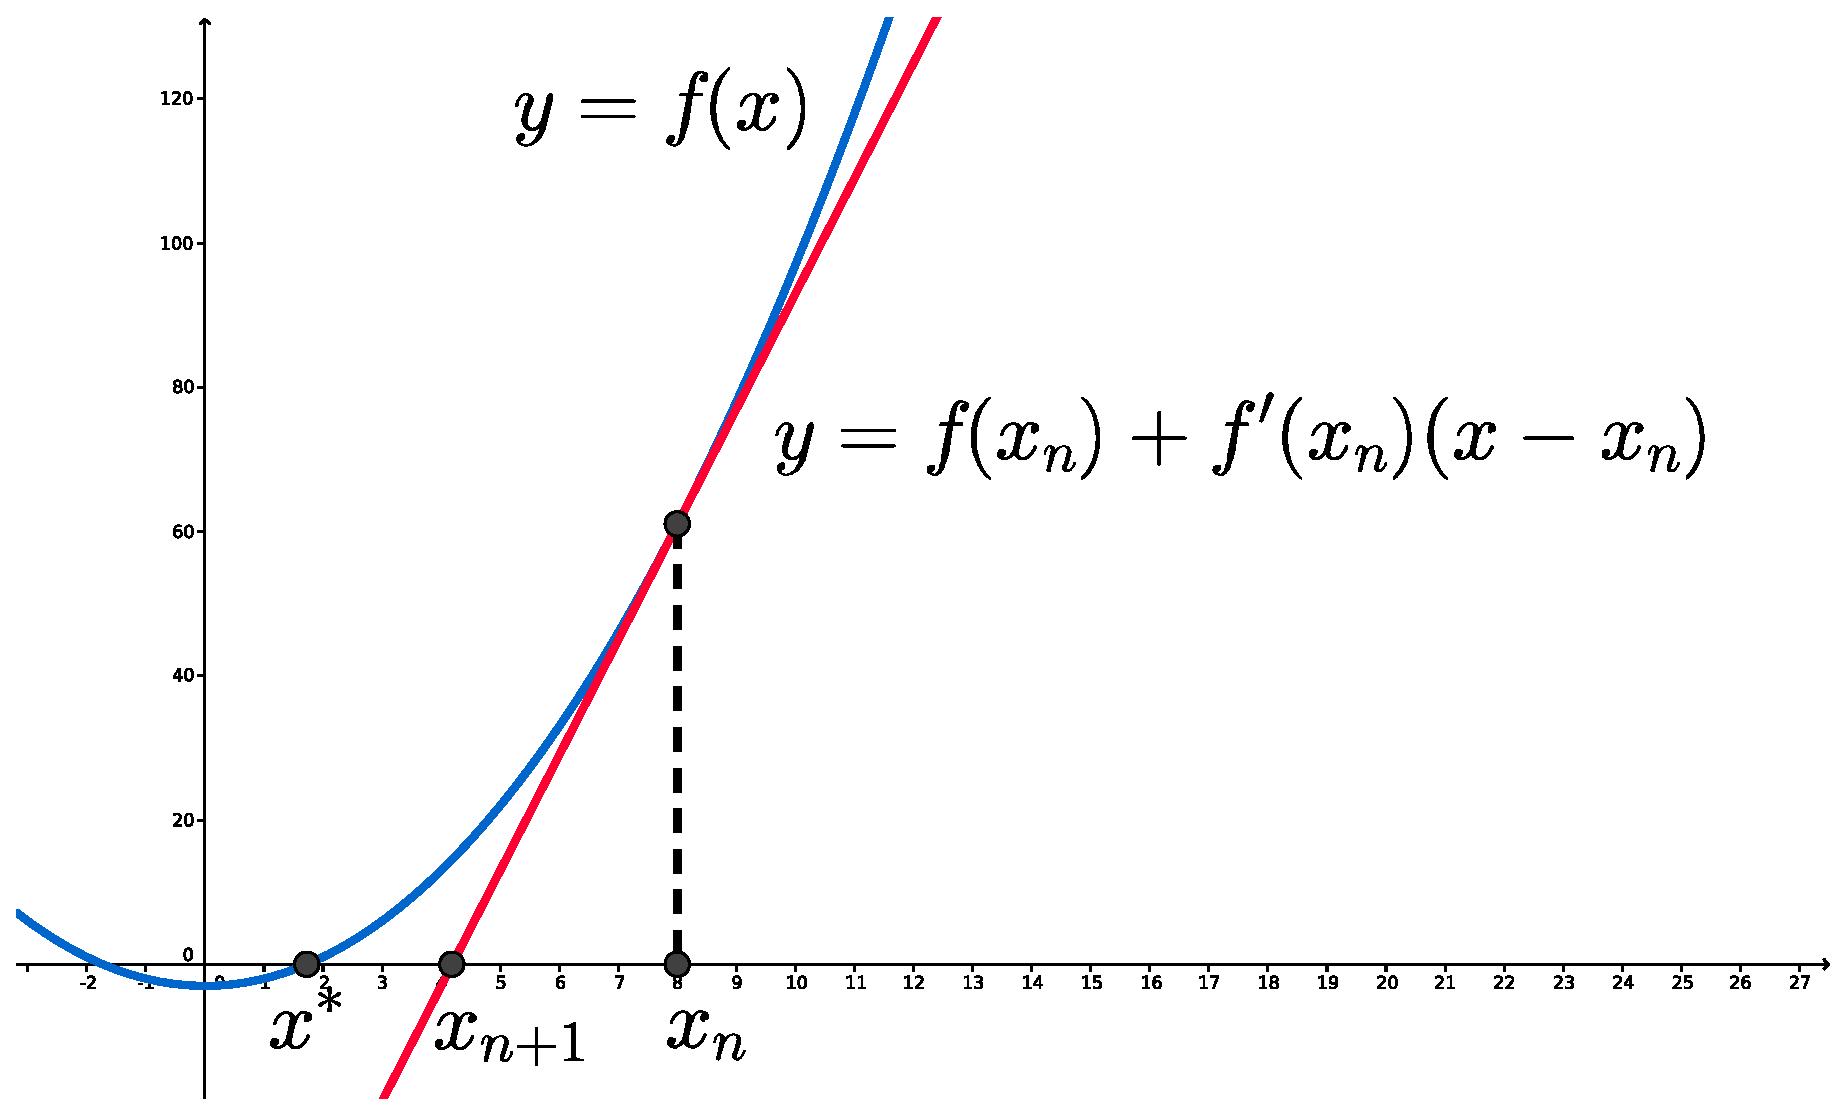
\includegraphics[scale=0.2]{./curva_newton.eps}
    \end{center}
    \caption{Interpretaci\'on geom\'etrica del m\'etodo de Newton.}
    \end{figure}
  \end{itemize}
\end{frame}
%%%%%
\begin{frame}
  \frametitle{Ejemplo}
  \begin{itemize}
    \item<1-> Se quiere aproximar uno de los ceros de la funci\'on $f(x) = \cos(x)\cosh(x) + 1$.
    Estableciendo una tolerancia de $10^{-8}$ y un n\'umero m\'aximo de 30 iteraciones, se obtiene:    
    \begin{table}[!ht]
    \begin{center}
      \small{
      \begin{tabular}{|c||c||c||c||c|}\hline
      $n$  & $x_n$ & $f(x_n)$ & $|x_n-x_{n-1}|$ \\\hline\hline
      0 & 8.000000000e+00 & -2.158647684e+02 & --------------- \\\hline
      1 & 7.872381323e+00 & -2.313725081e+01 & 1.276186774e-01 \\\hline
      2 & 7.855060668e+00 & -3.912804745e-01 & 1.732065443e-02 \\\hline
      3 & 7.854757530e+00 & -1.184721667e-04 & 3.031380765e-04 \\\hline
      4 & 7.854757438e+00 & -1.039879294e-11 & 9.183996408e-08  \\\hline  
    \end{tabular}}
     \caption{Resultados de resolver $\cos(x)\cosh(x) + 1=0$ mediante el m\'etodo de Newton.}
     \end{center}
     \label{tab_NR}
    \end{table}
  \end{itemize}
\end{frame}
%%%%%
\begin{frame}
  \frametitle{Posibles Problemas del M\'etodo de NR}
  \begin{itemize}
    \item<1-> El m\'etodo de Newton es uno de los m\'etodos m\'as usados para calcular numericamente raices de ecuaciones no
    lineales, pues si se escoge adecuadamente la aproximaci\'on inicial $x_0$, la sucesi\'on obtenida por iteraci\'on
    converge razonablemente r\'apido a la soluci\'on. 
    \item<2-> Sin embargo, este es un m\'etodo denominado local, pues si $x_0$ no es
    lo suficientemente cercano a $x^*$ y la funci\'on $f(x)$ no tiene ``buenas propiedades'', se pueden presentar algunos
    problemas. El siguiente ejemplo muestra algunas de las situaciones indeseables en el m\'etodo de Newton.    
  \end{itemize}
\end{frame}
%%%%%%
\begin{frame}
  \frametitle{Posibles Problemas del M\'etodo de NR}
  \begin{itemize}
    \item<1-> Considere el problema $f(x) = \sin(x) = 0$ en el intervalo $[-\pi/2, \pi/2]$. 
    \item<2->El m\'etodo de Newton es: dado $x_0 \in [-\pi/2, \pi/2]$, generar $\{x_n\}$ por medio de
  $$
  x_{n+1} = x_n - \frac{f(x_n)}{f'(x_n)} = x_n - \frac{\sin(x_n)}{\cos(x_n)} = x_n - \tan(x_n)
  $$
    \end{itemize}
  \end{frame}
  %%%%
  \begin{frame}
    \frametitle{Posibles Problemas del M\'etodo de NR}
    \begin{itemize}  
  \item Si se escoge $x_0 = \pi/2$, entonces $x_1 = -\infty$. De hecho, si escogemos $x_0$ cerca de $\pi/2$ \'o $-\pi/2$,
  la linea tangente intersecta al eje $x$ fuera del intervalo y muy lejos del mismo.
  \item<2-> Por ejemplo, tomando $x_0 = 1.4$ se
  obtiene $x_1 = -4.3979$.  
  \begin{figure}[ht]
  \begin{center}
    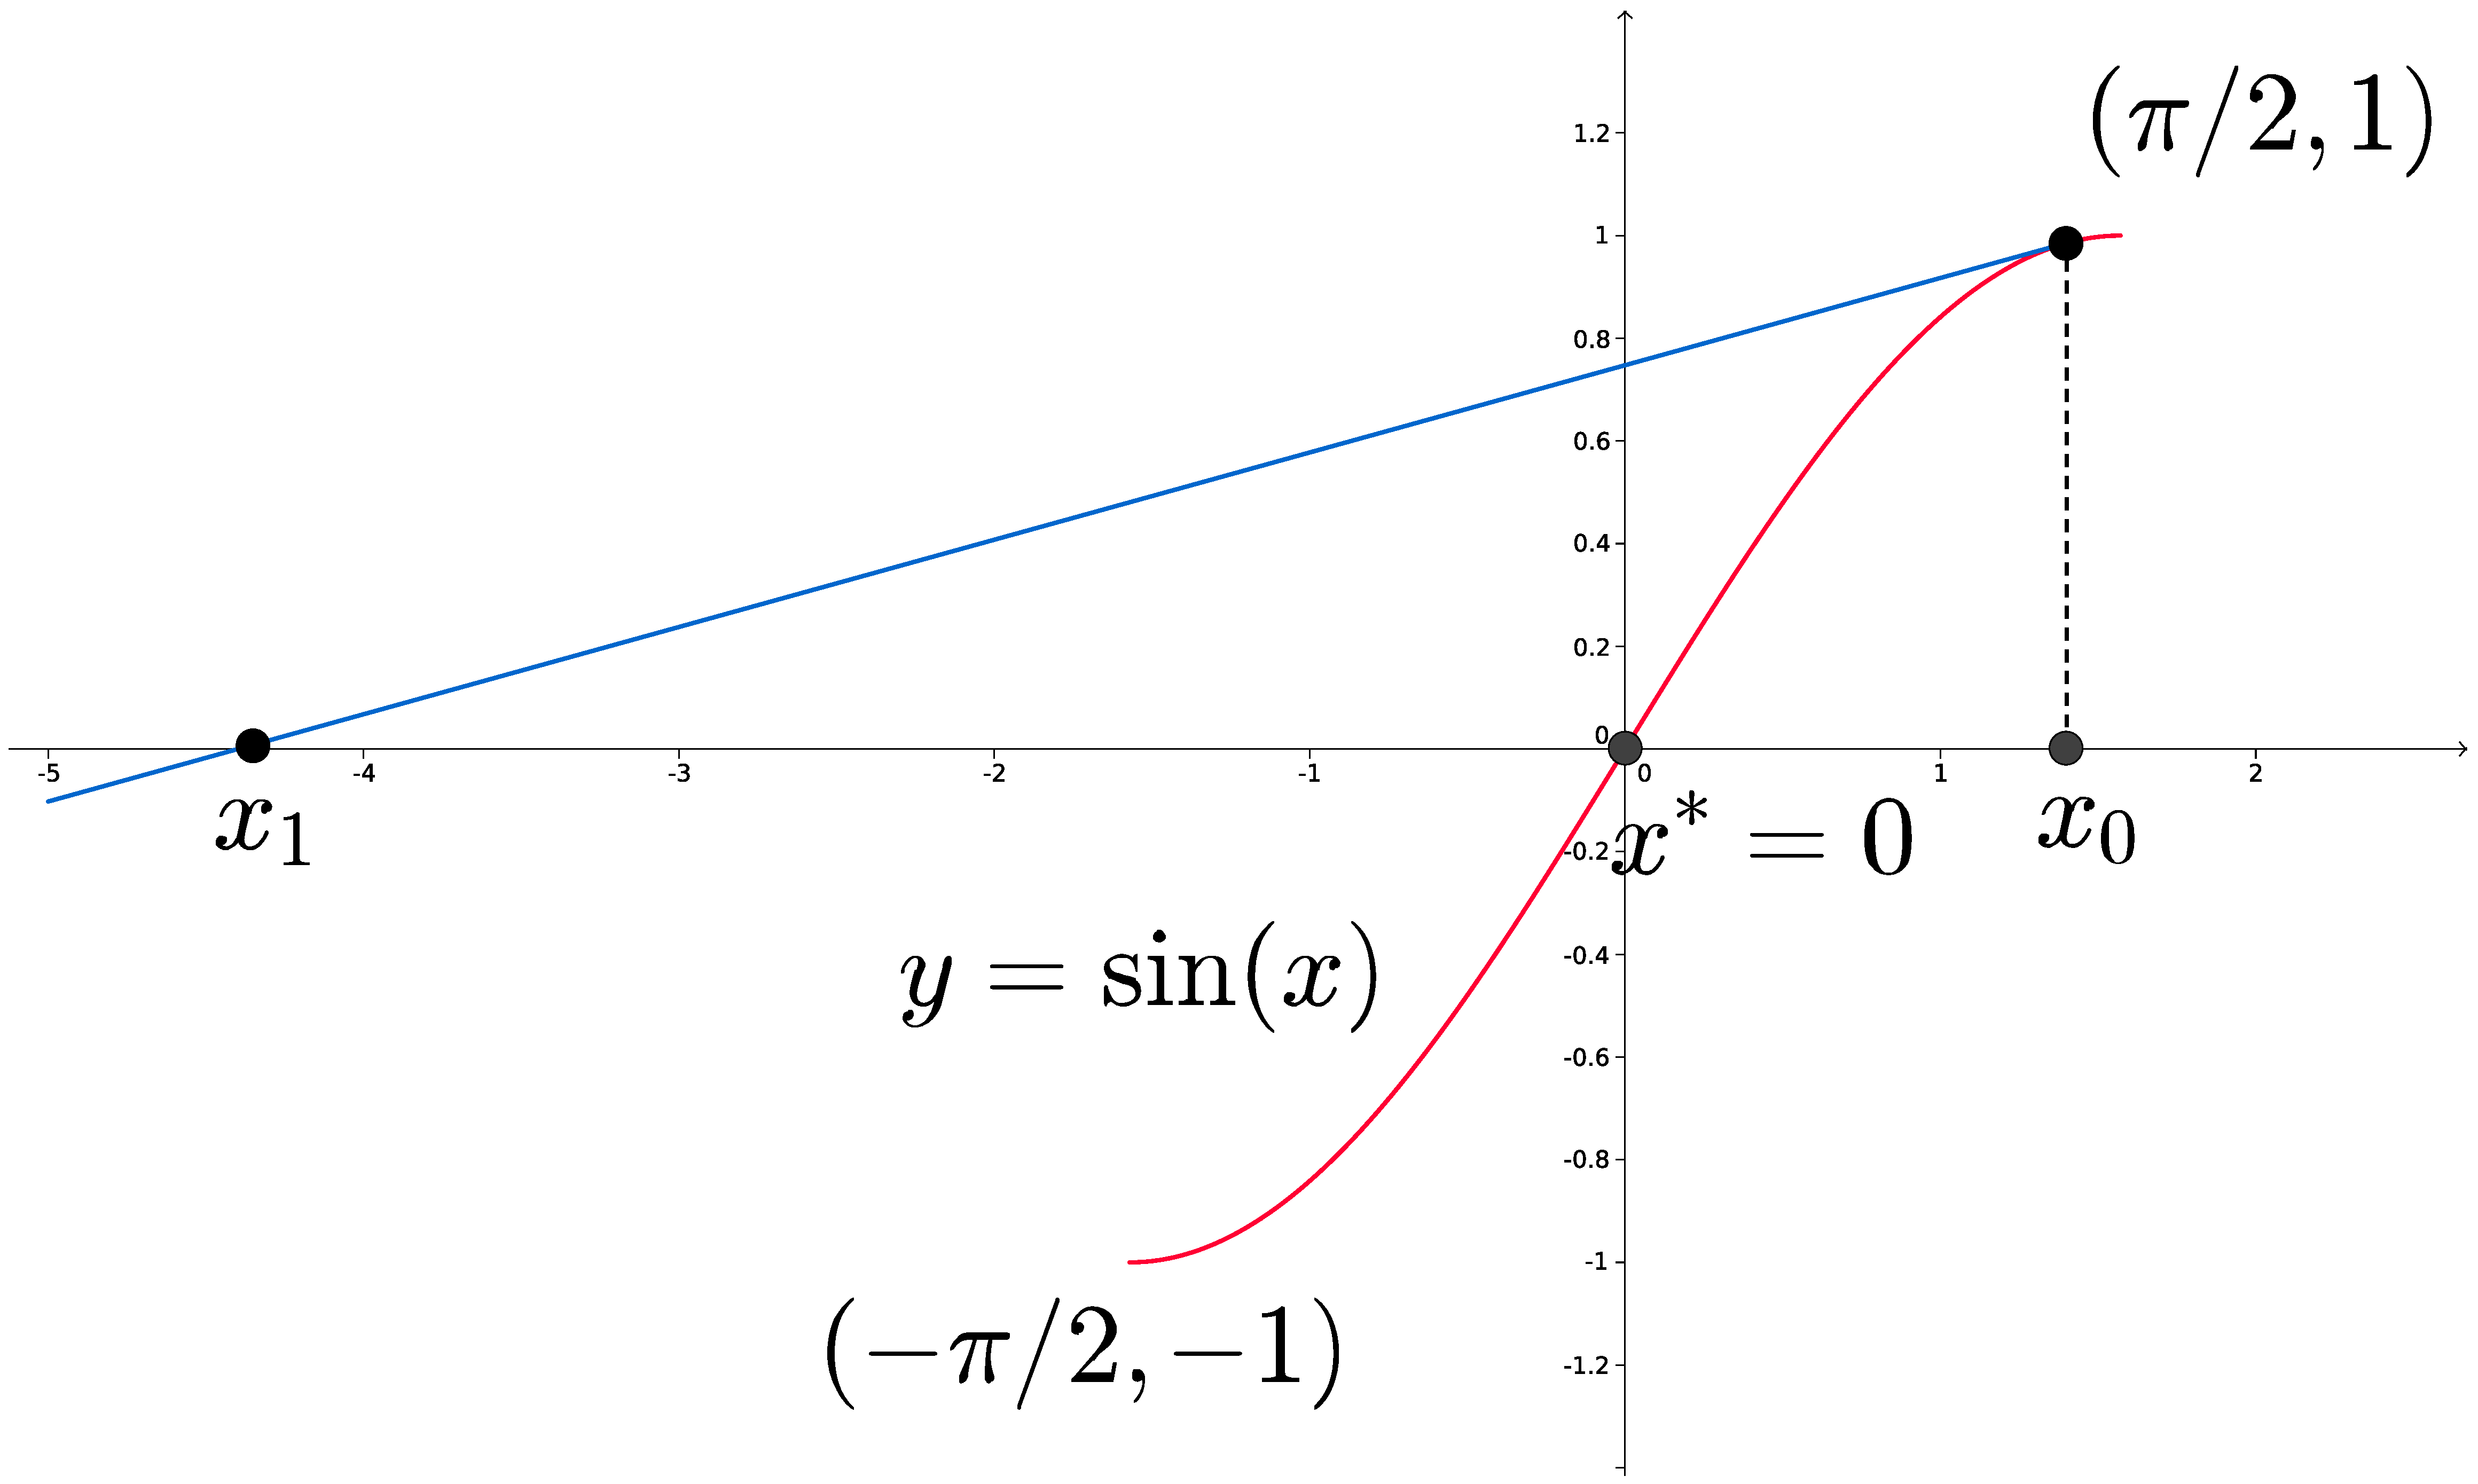
\includegraphics[scale=0.08]{./curva_newton_p1.eps}
  \end{center}
  \caption{Situaci\'on indeseable en el m\'etodo de Newton: $x_1$ cae muy lejos de $x^*$.}
  \end{figure} 
  \end{itemize} 
\end{frame}
%%%%%
\begin{frame}
  \frametitle{Posibles Problemas del M\'etodo de NR}
  \begin{itemize}
    \item<1-> Otro aspecto indeseable es que si escogemos $x_0 = x'$ tal que
    $$
    \tan(x') = 2x' \quad(x' \approx 1.1655\ldots),
    $$
    \item<2->entonces
    \begin{eqnarray}
    \nonumber x_1 & = & x_0 - \tan(x_0) = x_0 - 2x_0 = -x_0\\
    \nonumber x_2 & = & x_1 - \tan(x_1) = -x_0 - \tan(-x_0 ) = x_0
    \end{eqnarray}
    generando un ciclo obteniendo $x_0 , -x_0 , x_0 ,\ldots$ .    
    \begin{figure}[ht]
    \begin{center}
      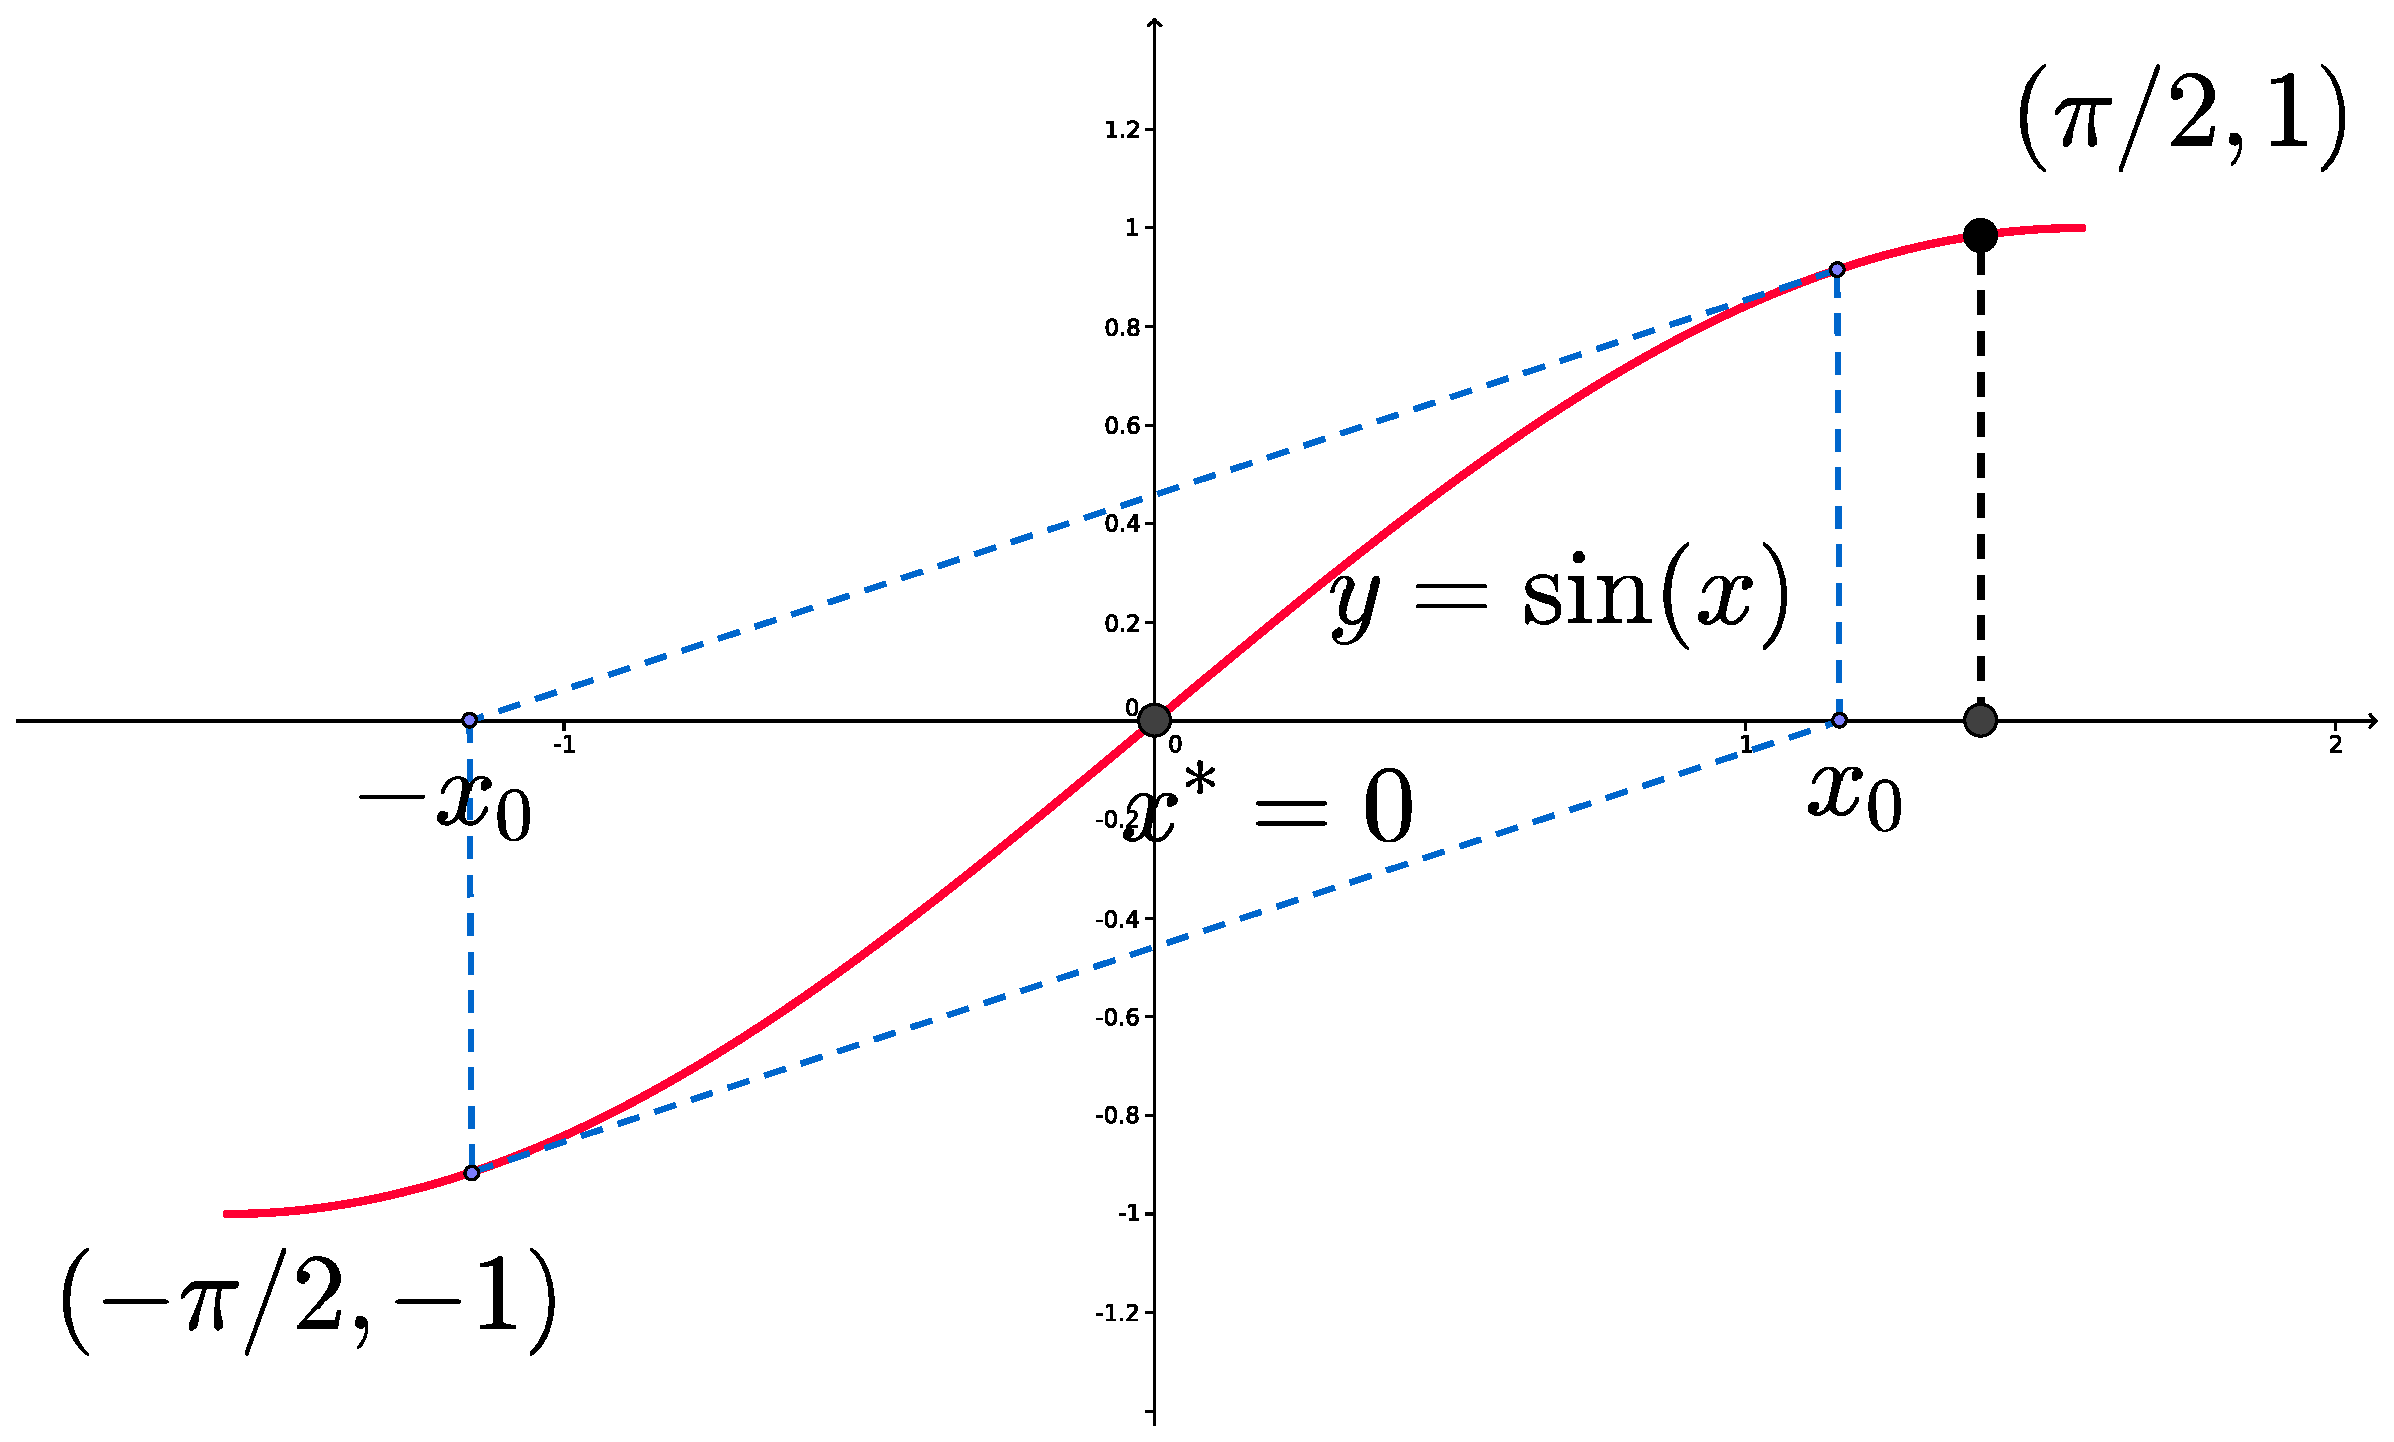
\includegraphics[scale=0.15]{./curva_newton_p2.eps}
    \end{center}
    \end{figure}    
  \end{itemize}
\end{frame}    
%%%%%
\begin{frame}
  \frametitle{Convergencia del M\'etodo de Newton-Raphson}
  \begin{itemize}
    \item<1-> El m\'etodo de Newton-Raphson es un m\'etodo de punto fijo,
    $$
    x_{n+1} = x_n - \frac{f(x_n)}{f'(x_n)} \equiv g(x_n)
    $$
    \item<2->El punto fijo para este m\'etodo es
    $$
    \alpha = \alpha - \frac{f(\alpha)}{f'(\alpha)} \Rightarrow f(\alpha)=0
    $$    
    es decir, una ra\'iz de $f(x)$.
    \item<3->En un entorno suficientemente peque\~no de $\alpha$, se cumple
    que el m\'etodo converge, ya que
    $$
    g'(x) = 1- \frac{f'(x)}{f'(x)} + \frac{f(x)f''(x)}{(f'(x))^2} = \frac{f(x)f''(x)}{(f'(x))^2}
    $$    
    implica que $g'(\alpha) = 0$, por lo que $|g'(x)| \ll 1$ en dicho entorno.
  \end{itemize}    
\end{frame}
%%%%%%
\begin{frame}
  \frametitle{Convergencia del M\'etodo de Newton-Raphson}
  \begin{itemize}
    \item<1-> Adem\'as, el m\'etodo de Newton tiene convergencia cuadr\'atica, ya que
    \small{
    \begin{eqnarray}
    \nonumber e_{n+1} & = & \alpha - x_{n+1} = \alpha - g(x_n)\\
    \nonumber & = & \underbrace{\alpha -g(\alpha)+g'(\alpha)(x_n-\alpha)}_{=0} - \frac{g''(\alpha)}{2}(x_n -
    \alpha)^2 - O((x_n - \alpha)^3)\\
    \nonumber & = & - \frac{g''(\xi)}{2}e_n^2 = Ce_n^2\\
    \nonumber & \Rightarrow & \frac{e_{n+1}}{e_n^2}  =  C
    \end{eqnarray}}
    \item<2-> donde $x_n \leq \xi \leq \alpha$ y lo que indica que el m\'etodo converge cuadr\'aticamente con $C$ como constante
    asint\'otica de error (es decir, su orden de convergencia es dos).
    \end{itemize}
  \end{frame}     
  %%%%%
\begin{frame}
  \frametitle{Algoritmo del M\'etodo de Newton-Raphson}
  \begin{algorithm}[H]
    \SetKwInOut{Input}{input}
    \SetKwInOut{Output}{output}
    \caption{Algoritmo de Newton-Raphson.}
    \Input{$x_0 \in \mathbb{R}$, N\'umero m\'aximo de iteraciones $N$, tolerancia $TOL$, funciones $f$ y $f'$.}
    \Output{Soluci\'on aproximada $p$ tal que $f(p)\approx 0$.}
    $i \leftarrow 1$\\
    \While{$i \leq N$}
    {
     $\displaystyle p \leftarrow x_0-\frac{f(x_0)}{f'(x_0)}$\\
     $i \leftarrow i +1$\\
     \If{$|p-x_0|<TOL$}
     {
       Salida($p$), \quad    EXIT\\
     }
     
     $x_0  \leftarrow p$\\
    }    
   \end{algorithm}
\end{frame}
%%%%%
\section{M\'etodo de la Secante}
\begin{frame}
  \frametitle{M\'etodo de la Secante}
  \begin{itemize}
    \item<1-> Una de las desventajas del m\'etodo de Newton es que en cada iteraci\'on hay que evaluar tanto a $f(x)$ como a $f'(x)$, para
    atenuar esa desventaja se propone el m\'etodo de la secante.
    \item<2-> En el m\'etodo de la secante se parte de dos puntos $(p_0,f(p_0))$ y $(p_1,f(p_1))$, por esos dos
    puntos pasa una secante que los une y cuya pendiente es    
    $$
    m = \frac{f(p_1) - f(p_0)}{p_1 - p_0}
    $$    
  \end{itemize}    
\end{frame}
%%%%%
\begin{frame} 
  \frametitle{M\'etodo de la Secante}
  \begin{itemize}
    \item<1-> Dado que esta recta secante corta al eje $x$ en el punto $(p_2 , 0)$, entonces tambi\'en se tiene que
    $$
    m = \frac{0 - f(p_1)}{p_2 - p_1}
    $$
    \item<2->luego entonces    
    $$
    m = \frac{f(p_1) - f(p_0)}{p_1 - p_0} = \frac{0 - f(p_1)}{p_2 - p_1}
    $$
    por lo tanto    
    $$
    p_2 = p_1 - \frac{f(p_1)(p_1 - p_0)}{f(p_1) - f(p_0)}
    $$
    \item<3->Este proceso genera la f\'ormula de iteraci\'on:    
    $$
    p_{k+1} = p_k - \frac{f(p_k)(p_k - p_{k-1})}{f(p_k) - f(p_{k-1})}
    $$
  \end{itemize}    
\end{frame} 
%%%%
\begin{frame}
  \frametitle{M\'etodo de la Secante}
  \begin{itemize}
    \item<1-> La siguiente imagen muestra un ejemplo de aplicaci\'on del m\'etodo de la secante para encontrar una ra\'iz de una funci\'on.
    \centering
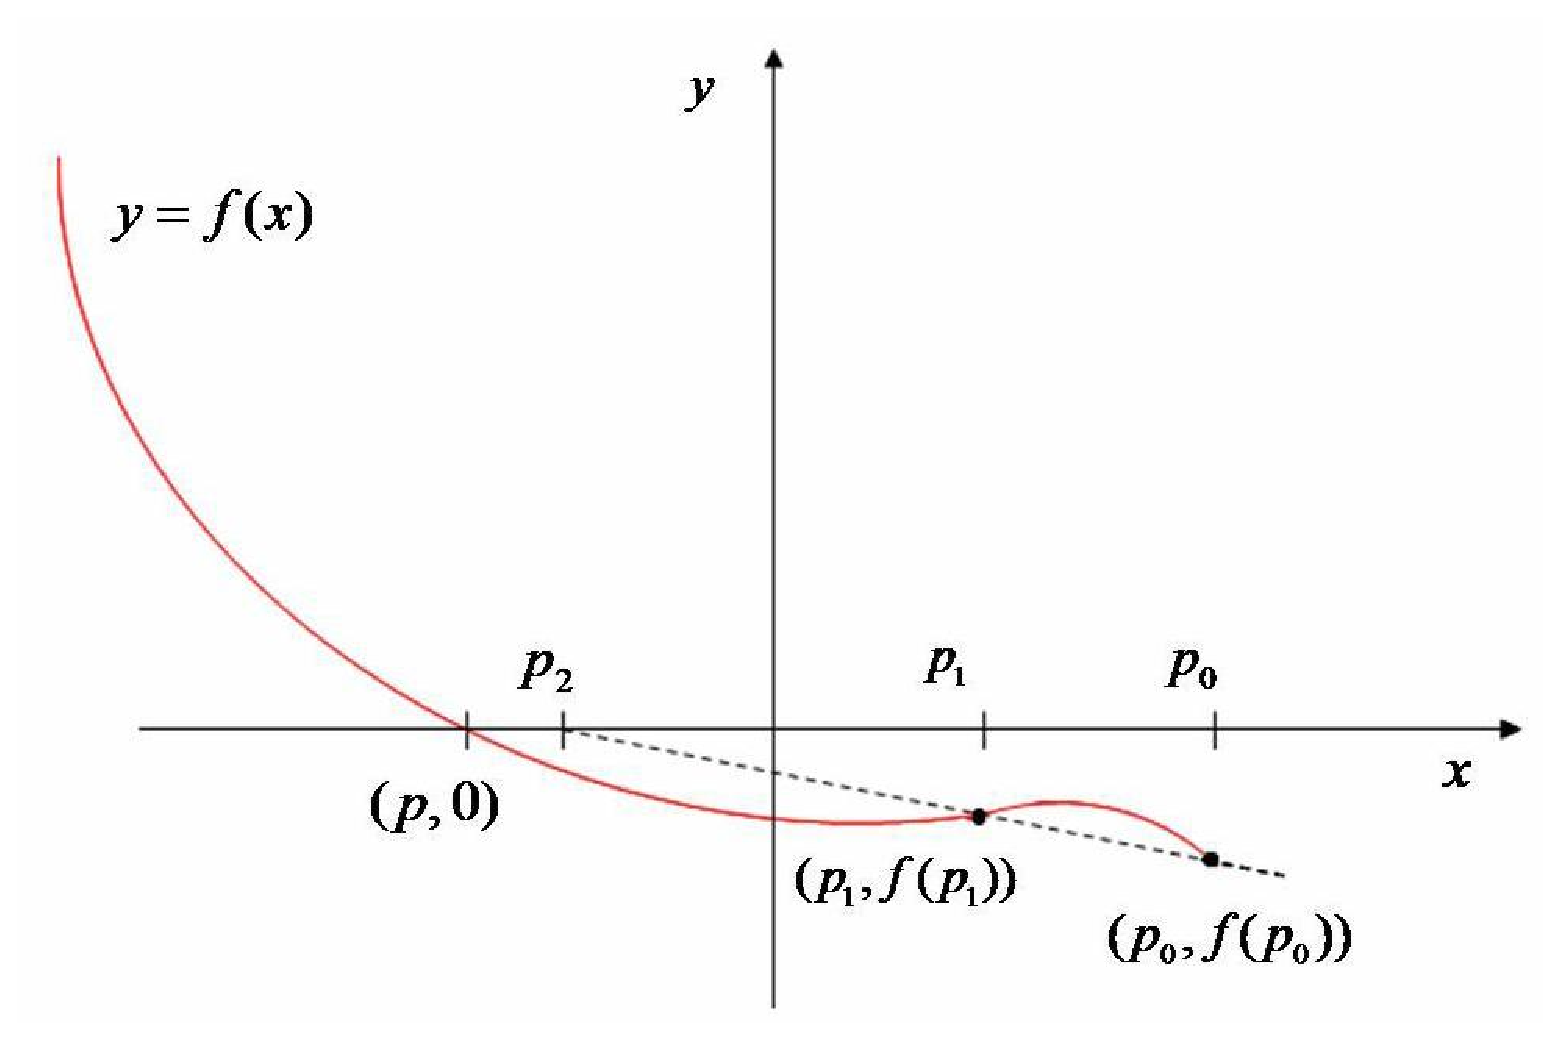
\includegraphics[scale=0.35]{sec1.eps}
  \end{itemize}    
\end{frame}
%%%%
\begin{frame}
  \frametitle{Convergencia del M\'etodo de la Secante}
  \begin{block}{Teorema}
    Sea $x^*$ un cero de $f(x)$ y supongamos que $f''(x^*) \neq 0$, entonces el orden de convergencia del m\'etodo de la secante es
$p=\frac{1}{2}(1+\sqrt{5})$.
  \end{block}
  \uncover<2->{
  \begin{block}{Demostraci\'on:}
    \small{
    Sea $e_k = p_k - x^*, \, k=0,1,2,\ldots$ como
    $$
      p_{k+1} = \frac{p_{k-1}f(p_k) - p_kf(p_{k-1})}{f(p_k) - f(p_{k-1})}
    $$
    \uncover<3->{
    $$
    \begin{array}{rcl}
      p_{n+1} - x^* & = & \dfrac{p_{n-1}f(p_n) - p_nf(p_{n-1})}{f(p_n) - f(p_{n-1})} -  \dfrac{x^*f(p_n) -
     x^*f(p_{n-1})}{f(p_n) - f(p_{n-1})} \\
      & = & \dfrac{(p_{n-1}-x^*)f(p_n) - (p_n - x^*)f(p_{n-1})}{f(p_n) - f(p_{n-1})}
     \end{array}
     $$}}
  \end{block}}
\end{frame}
%%%%%
\begin{frame}
  \frametitle{Convergencia del M\'etodo de la Secante}
  \begin{block}{Demostraci\'on:}
    De este modo:
    $$
    e_{n+1} = \frac{e_{n-1}f(x^*+e_n)-e_nf(e_{n-1}+x^*)}{f(x^*+e_n) - f(e_{n-1}+x^*)}
    $$
    \uncover<2->{
    pero por el desarrollo de Taylor de $f(x^* + e_n)$ y $f(x^* + e_{n-1})$ alrededor de $x^*$ se tiene que
    $$
    f(x^*+e_n) = f(x^*) + f'(x^*)e_n + \frac{1}{2}f''(x^*)e_n^2 + \cdots
    $$
    $$
    f(x^*+e_{n-1}) = f(x^*) + f'(x^*)e_{n-1} + \frac{1}{2}f''(x^*)e_{n-1}^2 + \cdots
    $$}
  \end{block}
\end{frame}  
%%%%%
\begin{frame}
  \frametitle{Convergencia del M\'etodo de la Secante}
  \begin{block}{Demostraci\'on:}
    pero como $f(x^*) = 0$ entonces,
    $$
    e_{n-1}f(x^*+e_n) = f'(x^*)e_ne_{n-1} + \frac{1}{2}f''(x^*)e_n^2e_{n-1} + \cdots
    $$    
    $$
    e_nf(x^*+e_{n-1}) = f'(x^*)e_{n-1}e_n + \frac{1}{2}f''(x^*)e_{n-1}^2e_n + \cdots
    $$
    \uncover<2->{
    adem\'as
    \small{
    $$
    f(x^*+e_n) - f(x^*+e_{n-1}) = f'(x^*)(e_n - e_{n-1}) + \frac{1}{2}f''(x^*)(e_n^2 - e_{n-1}^2) + \cdots
    $$}}
  \end{block}
\end{frame}
%%%%
%%%%%
\begin{frame}
  \frametitle{Convergencia del M\'etodo de la Secante}
  \begin{block}{Demostraci\'on:}
    de modo que
    $$
    e_{n+1} = \frac{\frac{1}{2}f''(x^*)e_ne_{n-1}(e_n-e_{n-1}) + \cdots}{f'(x^*)(e_n - e_{n-1})+ \cdots}
    $$
    \uncover<2->{
    para $|e_{n-1}|$ y $|e_n|$ suficientemente peque\~nos se tiene que
    $$
    e_{n+1} \approx \frac{f''(x^*)e_ne_{n-1}}{2f'(x^*)}
    $$}
    \uncover<3->{as\'i que
    $$
    |e_{n+1}| \approx M|e_ne_{n-1}| = M|e_n||e_{n-1}|
    $$
    siendo $M=\frac{f''(x^*)}{2f'(x^*)}$}
  \end{block}
\end{frame}
%%%%%
\begin{frame}
  \frametitle{Convergencia del M\'etodo de la Secante}
  \begin{block}{Demostraci\'on:}
    Pero se quiere obtener el valor de $p$, para el cual
    $$
    |x^* - x_n| = \alpha|x^* - x_{n-1}|^p \Rightarrow |e_n| = \alpha|e_{n-1}|^p
    $$
con $\alpha \geq 0,\, p \geq 1$, pero tambi\'en
$$
|e_{n+1}| = \alpha|e_{n}|^p = \alpha\left(\alpha|e_{n-1}|^p\right)^p
$$
\vspace{-0.25cm}
\uncover<2->{
As\'i que:
$$
\alpha^{p+1}|e_{n-1}|^{p^2} = M(\alpha|e_{n-1}|^p)|e_{n-1}|= \alpha M\left(|e_{n-1}|^{p+1}\right)
$$}
\uncover<3->{
la cual es v\'alida si $\alpha^p = M$ y $p^2 = p + 1$, de modo que
$$
p = \frac{1}{2}(1+\sqrt{5})
$$}
  \end{block}
\end{frame}
%%%%
\section{Aceleraci\'on de la convergencia de los m\'etodos iterativos: m\'etodo $\Delta^2$ de Aitken}
\frame{
\frametitle{Aceleraci\'on de la convergencia de los m\'etodos iterativos: m\'etodo $\Delta^2$ de Aitken}
Cuando el m\'etodo de resoluci\'on de ecuaciones no lineales que se est\'e empleando para resolver una ecuaci\'on
no lineal no posea convergencia, puede utilizarse la estrategia conocida con el nombre de m\'etodo delta-dos
($\Delta^2$) de A. C. Aitken para mejorar su velocidad de convergencia. 
\begin{block}{Definici\'on}
 Dada una sucesi\'on $\{x_i\}_i^{\infty}$ se denomina diferencia progresiva de primer orden en el punto $x_i$, y
se denota por $\Delta x_i$, al valor:
$$
\Delta x_i = x_{i+1} - x_i \qquad i\geq 0
$$
\end{block}
}
\frame
{
An\'alogamente se define la diferencia progresiva de orden $m$ en el punto $x_i$, y se denota por $\Delta^m x_i$, mediante:
$$
\Delta^m x_i = \Delta(\Delta^{m-1} x_i) \qquad i\geq0,m\geq2
$$
En concreto la diferencia progresiva de orden 2 ser\'a, seg\'un la definici\'on anterior:
$$
\Delta^2 x_i = \Delta(\Delta x_i) = \Delta x_{i+1} - \Delta x_i = x_{i+2} -2x_{i+1} +x_i, \qquad i\geq 0
$$
\begin{block}{Teorema}
 Sea $\{x_i\}_{i=0}^{\infty}$ una sucesi\'on convergente hacia $x^*$, y sea $\{y_i\}_{i=0}^{\infty}$ una nueva sucesi\'on generada a partir de la primera mediante:
$$
y_i = x_i - \frac{(\Delta x_i)^2}{\Delta^2x_i} = \frac{x_ix_{i+2}-x_{i+1}^2}{x_{i+2} -2x_{i+1} +x_i}, \qquad i\geq0
$$
entonces la sucesi\'on $\{y_i\}_{i=0}^\infty$ converge hacia $x^*$. 
\end{block}
}

% %%%%
\begin{frame}[fragile]
Dada la ecuaci\'on $x = g(x)$, el indicador de precisi\'on $tol$, un valor m\'aximo de iteraciones a realizar ($maxiter$) y un punto $p_0$ 
\small
\begin{verbatim}
 Entrada: g,p0,tol,maxiter
 Salida: Solucion aproximada o mensaje de error
     p1=g(p0)
     Mientras (i <= maxiter)
           p2=g(p1)
           p=p2 - (p2-p1)^2/(p2-2p1+p0)           
           i = i + 1;
           si |p-p0| < tol entonces
              salida(p)
              PARAR
           fsi
           p0=p1
           p1=p2
     fmientras
 salida: “fracaso busqueda # max de iters excedido”
\end{verbatim}
\end{frame}
% %%%%
\section{M\'etodo de Steffensen}
\frame
{
\frametitle{M\'etodo de Steffensen}
Todo lo anterior puede utilizarse para elaborar un algoritmo que mejore la velocidad de convergencia de los m\'etodos de
orden de convergencia inferior a 2. Este algoritmo conocido tambi\'en con el nombre de m\'etodo de Steffensen,
se muestra a continuaci\'on:
}
%%%%
\begin{frame}[fragile]
Dada la ecuaci\'on $x = g(x)$, el indicador de precisi\'on $tol$, un valor m\'aximo de iteraciones a realizar
($maxiter$) y un punto $p_0$ 

\small
\begin{verbatim}
 Entrada: g,p0,tol,maxiter
 Salida: Solucion aproximada o mensaje de error
     Mientras (i <= maxiter)
           p1=g(p0)
           p2=g(p1)
           p=p2 - (p2-p1)^2/(p2-2p1+p0)
           i = i + 1;
           si |p-p0| < tol entonces
              salida(p)
              PARAR
           fsi
           p0=p
     fmientras
 salida: “fracaso busqueda # max de iters excedido”
\end{verbatim}
\end{frame}
% %%%%
\frame{
\frametitle{Caracter\'isticas}
\begin{itemize}
 \item<1-> El m\'etodo es visto como m\'etodo de punto fijo $x= g (x)$ donde $g$ es indeterminada para $x= \alpha$ (punto fijo).
 \item<2-> Se puede calcular su orden de convergencia calculando $g'(\alpha)$. Pero el c\'alculo directo lleva a una indeterminaci\'on del tipo $0/0$ y se procede a resolver por otras t\'ecnicas. 
 \item<3-> Se usa un punto inicial $x_0$, luego se calcula $x_1$ a partir de una iteraci\'on representada por $g(x_0)$ y luego $x_2$ calculado a partir de otra iteraci\'on $g(x_1)$
\end{itemize}
}
% %%%%
\frame{
\frametitle{Ventajas}
 
\begin{itemize}
 \item<1-> Presenta una convergencia r\'apida hacia la ra\'iz y no requiere de evaluaci\'on de las derivadas.
 \item<2-> El proceso de iteraci\'on solo necesita un punto inicial $x_0$
 \item<3-> Se usa para acelerar la funci\'on de orden lineal, ya que converge la misma en una cuadr\'atica
\end{itemize}
}
%%%%
\frame{
\frametitle{Desventajas}
\begin{itemize}
 \item<1-> Requiere que $g'(\alpha) \neq 0$, condici\'on que es equivalente a requerir que la multiplicidad de la ra\'iz sea uno. Como consecuencia se puede esperar que el m\'etodo acelere de cuadr\'atico a la convergencia lineal.
 \item<2-> La debilidad fundamental del m\'etodo es la elecci\'on del valor inicial $x_0$. Si el valor no se aproxima a la soluci\'on, el m\'etodo puede fallar y la secuencia de los valores divergen al infinito.
 \item<3-> Tarda mucho a la hora de realizar las evaluaciones por medio de programas de c\'omputo.
\end{itemize}
}
\end{document}